\documentclass[a4paper, 12pt, english]{article}


% \usepackage[portuges]{babel}
\usepackage{fontspec}

\usepackage[utf8]{inputenc}
\usepackage{amsmath,amssymb}
\usepackage{graphicx}
\usepackage{subfig}
\usepackage[colorinlistoftodos]{todonotes}
\usepackage{longtable}  % For tables that span multiple pages
\usepackage{indentfirst}
\usepackage{verbatim}
\usepackage{textcomp}
\usepackage{gensymb}
\usepackage{braille}
\usepackage{relsize}
\usepackage{caption}
\usepackage{tabularray}
\usepackage{subcaption}  % For subfigures
\usepackage{lipsum}% http://ctan.org/pkg/lipsum
\usepackage{xcolor}% http://ctan.org/pkg/xcolor
\usepackage{xparse}% http://ctan.org/pkg/xparse
\usepackage{float} % Include this package for the [H] option
\usepackage{changepage} % for adjustwidth environment
\usepackage{xcolor}
\usepackage{ulem}

\NewDocumentCommand{\myrule}{O{1pt} O{2pt} O{black}}{%
  \par\nobreak % don't break a page here
  \kern\the\prevdepth % don't take into account the depth of the preceding line
  \kern#2 % space before the rule
  {\color{#3}\hrule height #1 width\hsize} % the rule
  \kern#2 % space after the rule
  \nointerlineskip % no additional space after the rule
}
\usepackage[section]{placeins}

\usepackage{booktabs}
\usepackage{colortbl}%
   \newcommand{\myrowcolour}{\rowcolor[gray]{0.925}}
   
\usepackage[obeyspaces]{url}
\usepackage{etoolbox}
\usepackage[colorlinks,citecolor=black,urlcolor=blue,bookmarks=false,hypertexnames=true]{hyperref} 

\usepackage{geometry}
\geometry{
	paper=a4paper, % Change to letterpaper for US letter
	inner=3cm, % Inner margin
	outer=3cm, % Outer margin
	bindingoffset=.5cm, % Binding offset
	top=2cm, % Top margin
	bottom=2cm, % Bottom margin
	%showframe, % Uncomment to show how the type block is set on the page
}
%*******************************************************************************%
%************************************START**************************************%
%*******************************************************************************%
\begin{document}

%************************************TITLE PAGE**************************************%
\begin{titlepage}
\begin{center}
\textbf{\LARGE ALEXANDRIA UNIVERSITY}\\[0.5cm] 
\textbf{\large FACULTY OF ENGINEERING}\\[0.2cm]
\vspace{20pt}

\includegraphics[scale=0.15]{AlexuLogo.png}\\[1cm]

\par
\textbf{ELECTRICAL ENGINEERING DEPARTMENT}\\
\vspace{15pt}
\textbf{\Large COMMUNICATION AND ELECTRONICS ENGINEERING PROGRAM}
\vspace{15pt}
\myrule[1pt][7pt]
\textbf{\LARGE  Optical Braille Translator}\\
%\vspace{15pt}
%\textbf{\large Signal Transmission $\&$ Distortion}\\
\myrule[1pt][7pt]
\vspace{25pt}

\textbf{\large Prepared by:}\\[0.2cm]

Abdallah Ashraf\\
Adham Mohamed\\
Ahmed Elsayed\\
Ali Elneklawy\\
Ayman Feteha\\
Nada Tarek\\
Nada Gamal\\

\vspace{45pt}
\textbf {\large Supervised by:}\\[0.2cm]
\Large {Dr. Mohamed Moselhy}\\[0.1cm]
\end{center}

\par
\vfill
\begin{center}
\textbf{ACADEMIC YEAR 2023/2024}\\
\end{center}

\end{titlepage}
\newpage
\textbf{\large Abstract}\\

This project addresses the challenge of accessibility for visually impaired individuals by focusing on the translation of Braille text into both printed text and speech. With millions of visually impaired individuals relying on Braille, there is a significant need for technology that bridges the gap between Braille literacy and digital accessibility. The primary objective of this project is to develop an inexpensive system that requires minimal user interaction, accurately translating scanned single-sided Braille pages into printed text and subsequently converting the text into speech. The project employs a dual-method approach for Optical Braille Recognition (OBR): the first using image processing techniques, and the second utilizing a Convolutional Neural Network (CNN). The process begins with the preprocessing of Braille pages, followed by the detection of Braille symbols through image processing techniques. These symbols are then recognized using both methods and converted into corresponding printed text. Finally, text-to-speech technology is used to convert the printed text into natural-sounding speech output. The developed system demonstrates high accuracy in translating Braille to text.  Our OBR system not only provides high accuracy but also ensures reliability, efficiency, and affordability. Additionally, we introduce a new Braille dataset containing annotated images of Braille symbols. This project successfully creates a robust tool for translating Braille into text and speech, significantly improving accessibility for the visually impaired community. The system facilitates easier access to written content and promotes greater independence and inclusion. Future enhancements could focus on expanding language support and integrating the system with mobile devices. \\
\\ \textbf{Keywords:} Optical Braille Recognition (OBR), Image processing, Convolutional Neural Network (CNN), text-to-speech, Braille Dataset.


\newpage
\textbf{\large Acknowledgements}\\


We would like to express our heartfelt gratitude to the following individuals, organizations, and entities who have contributed to the completion of our graduation project:

\begin{itemize}
    \item Alexandria University, Faculty of Engineering, for providing the necessary resources and environment conducive to learning and research.
    \item Dr. Mohamed Moselhy, our supervisor, for his invaluable guidance, support, and expertise throughout this project.
    \item The developers and contributors of the following software libraries and tools: PyQt5, TensorFlow, NumPy, OpenCV, Qt. These tools have been instrumental in the implementation and success of our project.
    \item The authors of the Tacotron paper, whose innovative work laid the foundation for our exploration into speech synthesis.
    \item AI Forever for the T5 Large model, which significantly enhanced the quality and efficiency of our natural language processing tasks.
    \item The institute supporting the visually impaired in the Faculty of Commerce at Alexandria University, especially for providing us with essential Braille materials. These materials enabled us to construct a comprehensive Braille characters dataset, contributing significantly to our research.
    \item Our team members, whose dedication, collaboration, and diverse skills have been pivotal in every phase of this project. Each team member's contribution has been essential to our success.
    \item Our friends and families, for their unwavering support, understanding, and encouragement throughout our academic journey.
\end{itemize}

\textit{We extend our sincere appreciation to everyone who has been part of this collective effort. Your contributions have made a lasting impact.}


%************************************TABLE OF CONTENTS**************************************%
\newpage
\hypersetup{linkcolor=black}
\tableofcontents
%  %Sumário
%  \newpage
%  \tableofcontents
%  \thispagestyle{empty}
%  %End Sumário

%********************************%
%***********SECTION 1************%
%********************************%
\newpage
\newpage
\section{{Introduction}
}




Braille is a tactile writing system used by people who are visually impaired. It was invented by Louis Braille in the early 19th century and has since become a vital tool for enabling blind and visually impaired individuals to read and write independently. The Braille system consists of patterns of raised dots arranged in cells of up to six dots in a 3x2 grid. Each pattern, or cell, represents a letter, number, punctuation mark, or even a word or a part of a word in many languages. An example of a Braille cell configuration is shown in figure 1.1.

% Set the figure counter to 0 (so the next figure is 1)
\setcounter{figure}{0}
% Redefine the figure numbering to be 1.<figure number>
\renewcommand{\thefigure}{1.\arabic{figure}}

\begin{figure}[h]
\centering
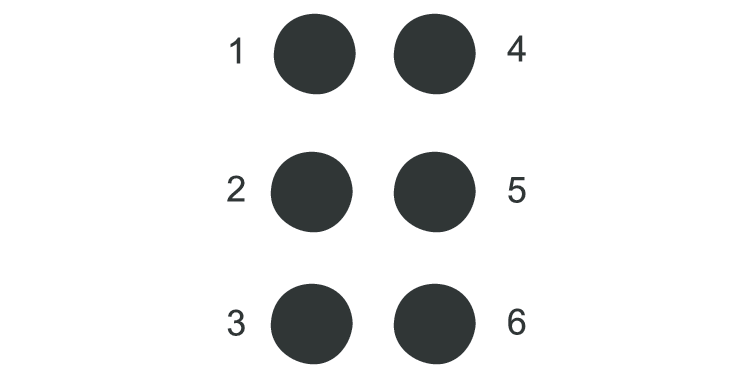
\includegraphics[width=0.5\textwidth]{Braille-six-dot-cell.png}
\caption{Braille Cell}
\label{fig:example}
\end{figure}


Braille is not a language in itself but rather a code that can be used to write any language. Each cell can be combined in various ways to form the letters of the alphabet, numbers, and other symbols. For example, the first ten letters of the alphabet are created using the top four dots of the Braille cell, while the remaining letters are formed by adding the fifth and sixth dots. Additionally, specific dot patterns are used to signify numbers and punctuation.

Braille literacy is crucial for the personal and educational development of individuals with visual impairments. It provides them with the means to access written information, pursue education, and engage in a wide range of professional activities. Moreover, it enhances their independence and ability to participate fully in society.

There are different grades of Braille, each serving a specific purpose. Grade 1 Braille, also known as uncontracted Braille, is a straightforward transcription where each Braille cell corresponds directly to an individual letter, number, or punctuation mark. It is often used for beginners who are just learning to read and write in Braille. Grade 1 alphabet and numbers is shown in figure 1.2. Grade 2 Braille, or contracted Braille, involves the use of contractions to represent common words or groups of letters, allowing for more efficient reading and writing. Contracted Braille is commonly used in books, signage, and other written materials to save space and make reading quicker. Figure 1.3 shows some of the most common words represented in grade 2.[13]

\renewcommand{\thefigure}{1.\arabic{figure}}

\begin{figure}[h]
\centering
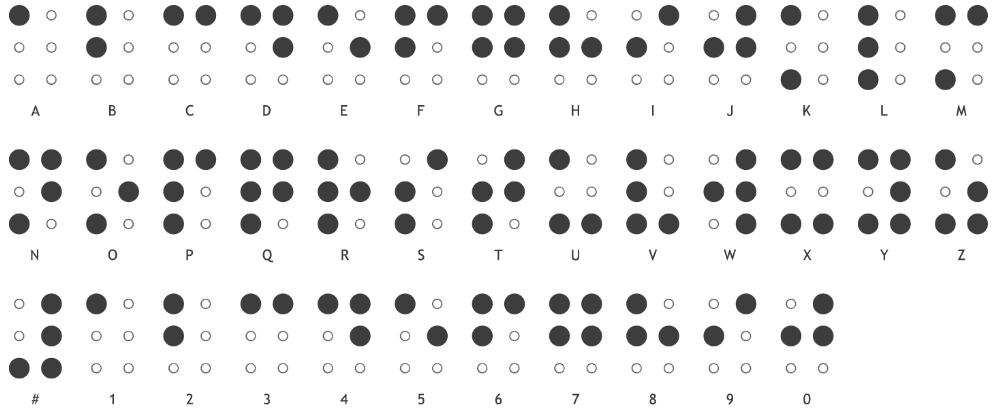
\includegraphics[width=0.9\textwidth]{alphabet_numbers.jpg}
\caption{Grade 1 Braille alphabet and numbers}
\label{fig:example}
\end{figure}

\begin{figure}[h]
\centering

\includegraphics[width=0.6\textwidth]{grade2.jpg}
\caption{Common grade 2 Braille words}
\label{fig:example}
\end{figure}


Despite its importance, the availability of Braille materials is limited. Producing Braille books and resources is a complex and costly process, which contributes to the scarcity of accessible materials for the visually impaired. This lack of resources highlights the need for innovative solutions that can bridge the gap between Braille literacy and accessibility. Our project, the "Optical Braille Translator," aims to address this need by providing a system that translates Braille into English text and converts it into audible speech, thereby enhancing access to Braille content and supporting the literacy and independence of visually impaired individuals.

\subsection{Problem Statement}


Braille literacy is crucial for individuals with visual impairments, as it provides them with the ability to read and write independently. Despite its importance, the accessibility and usability of Braille materials pose some challenges. The primary problem this project addresses is that converting printed text into Braille or vice versa is a labor-intensive process. Moreover, individuals who are not proficient in Braille find it difficult to access Braille content. The accessibility of braille content to for everyone is so important. Braille language is the way visually impaired people would express themselves or their thought. It is the way to introduce their cultural production to the world.


Other challenges that further complicate the issue, as non-Braille users, including family members, educators, and caregivers, struggle to engage with Braille content, limiting the support they can offer to visually impaired individuals. The isolation experienced by those who rely on Braille due to the communication gap with non-Braille users highlights the need for inclusive solutions.

Additionally, students with visual impairments face difficulties in mainstream educational environments due to the scarcity of accessible Braille materials. Teachers without Braille proficiency are unable to provide adequate instructional support, impacting the quality of education for visually impaired students. 

A specific problem this project aims to solve is the correction of high school final exams for students using Braille. Exam papers must be transported to the capital for correction, risking partial or full damage during the journey. Moreover, the process involves individuals not knowledgeable enough about the academic content translating from Braille to text, followed by correction by another individual, which increases the probability of human errors. By addressing these issues, the project seeks to create a system that enhances the accessibility and usability of Braille materials, fostering greater inclusion and independence for individuals with visual impairments.

All the previous raises the need for a system that can make Braille content easily accessible to everyone, including those without Braille literacy skills.


\subsection{Project Overview}


Our project aims to solve this problem by developing a system that leverages image processing and deep learning techniques to facilitate the translation of scanned Braille images into English text. Additionally, the system converts the extracted text into audible speech, enhancing accessibility for visually impaired individuals. The project focuses on translating grade 1, front-only, scanned Braille images.

The system is designed to be user-friendly, ensuring that individuals with varying levels of technical expertise can use it effectively. Our project provides a solution that not only interprets Braille characters accurately but also synthesizes the extracted text into speech. This dual functionality makes Braille content more accessible and usable for a broader audience.

\subsubsection{Objectives}

The primary objective of our project is to develop a Braille to text translation system that can accurately detect and recognize Braille characters from scanned images using image processing and deep learning techniques. To further enhance the usability of the system, we aim to integrate a text-to-speech conversion feature that transforms the extracted English text into audible speech, making it accessible to individuals who cannot read Braille. Ensuring high accuracy and usability is another key objective, as we strive to design the system to achieve high accuracy in Braille recognition while providing a user-friendly interface for easy operation. Ultimately, the project seeks to enhance accessibility by enabling visually impaired individuals and those without Braille literacy skills to access Braille content effortlessly.

\subsubsection{Methodology}

To achieve these objectives, our project employs a multi-step approach. The scanned Braille images undergo preprocessing filters to enhance image quality and prepare the digital image for analysis. This step includes noise reduction, normalization, and page alignment. 



The system utilizes image processing techniques to detect Braille characters using two different methods: dot detection using Hough circle transformation(HCT) or detection of symbols using white spaces between the symbols and dividing the page to individual symbols. 

The next step is recognize the symbols using again two approaches: grid formation or using CNN to recognise the symbols from the divided image .

The recognized Braille characters are translated into English text, and a text correction module is employed to ensure the accuracy and coherence of the translated text. 

The corrected text is then converted into audible speech using a text-to-speech engine, providing an auditory output of the Braille content.

Finally, a graphical user interface (GUI) is developed to facilitate easy interaction with the system, and extensive testing is conducted to evaluate the system's performance and accuracy. Each of these steps will be explained in detail in the upcoming chapters.

\begin{figure}[!ht]
\centering
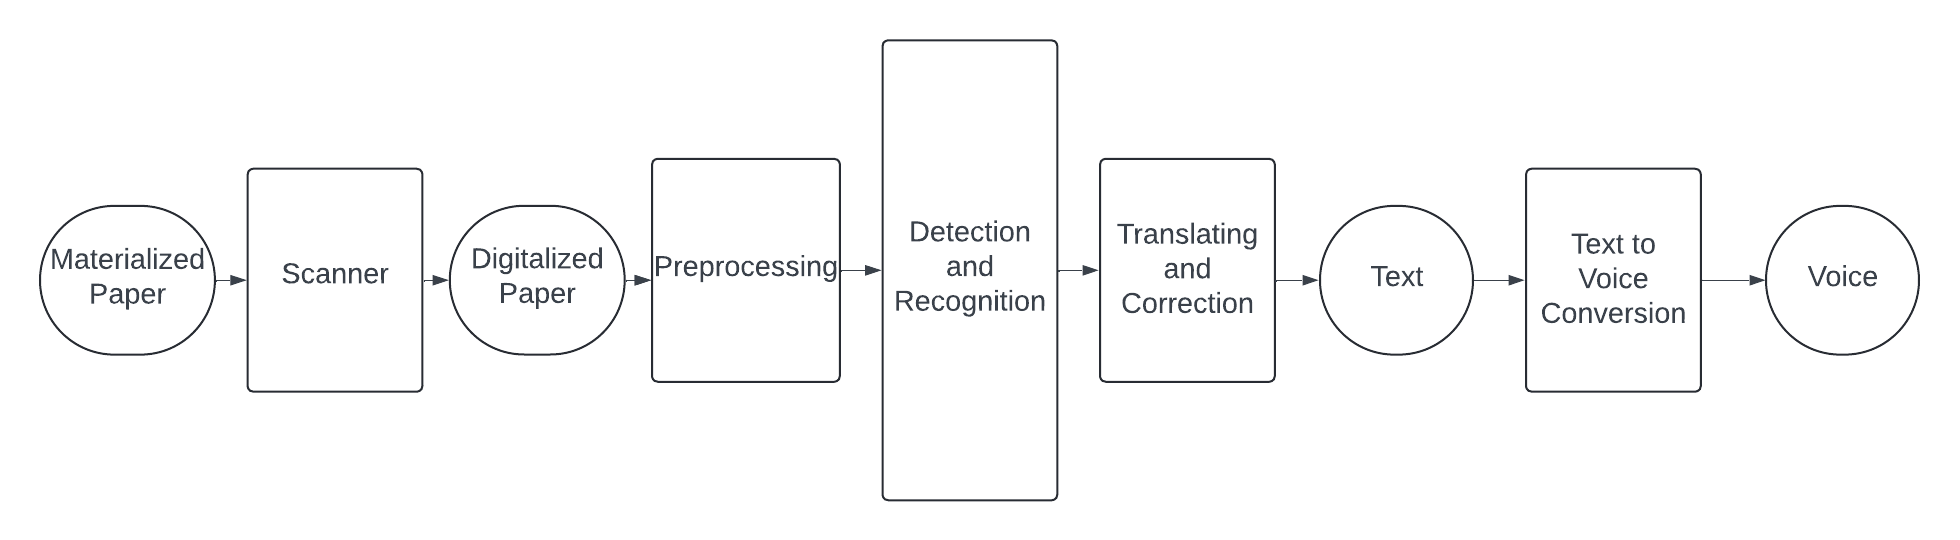
\includegraphics[width=1\linewidth]{Block diagram.png}
\caption{Block Diagram}
\label{fig:Block Diagram}
\end{figure} 

\subsubsection{Conclusion}

In conclusion, our project addresses a critical need in the realm of accessibility for visually impaired individuals. By combining image processing, deep learning, and text-to-speech technologies, we have developed a comprehensive solution that translates Braille into English text and converts it into audible speech. This innovative system not only enhances Braille literacy but also makes Braille content accessible to a wider audience, thereby bridging the gap between Braille literacy and accessibility.

The following chapters will delve into the technical details of the project, including the system design, preprocessing techniques, detection and recognition methods, and the implementation of text-to-speech conversion. Through this comprehensive exploration, we aim to provide a thorough understanding of the project's development and its impact on enhancing accessibility for visually impaired individuals.

%********************************%
%***********SECTION 2************%
%********************************%
\newpage
\section{Literature review}

As discussed before, this project aims to develop a system for optical Braille character detection, translation to English text, correction of the text, and finally conversion of the text to speech. This literature review examines existing research and technologies in Optical Braille Character Recognition (OBR), Braille recognition and translation, text correction algorithms, and text-to-speech (TTS) systems, highlighting their relevance and application to this project.\\


\subsection{Optical Braille Character Recognition (OBR)}

Numerous studies have addressed the problem of optical Braille detection, leading to the development of various methods for detecting and translating Braille into text. Over the years, continuous research has significantly improved accuracy, approaching near perfection. This progress has been achieved through techniques such as object detection using support vector machines, various image processing steps and filters, and machine learning, particularly with the recent advancements in artificial intelligence (AI) and deep learning.
\\
In this section, we will discuss some of these methods. We will begin with the image preprocessing steps and the filters employed in previous research.

\textbf{
\subsubsection{Image Acquisition}
}
Different mechanisms for image acquisition have been proposed in various studies. For instance, the paper titled "Image Processing Techniques for Braille Writing Recognition" by Néstor Falcón et al. [1] highlights the use of a flat-bed scanner instead of a digital camera. The choice of a flat-bed scanner is justified by its cost-effectiveness, versatility for other applications, and ease of use. The system described in the paper is capable of working with images of different resolutions, specifically adjusting images through interpolation methods to resize input images to a standard resolution, typically around 100 dots per inch (dpi). 

In the study titled "Analysis of Scanned Braille Documents" by Ritchings et al. [12], the methodology for optical Braille detection involves scanning Braille documents at 100 dpi to produce gray-scale images with 16 levels. This configuration was selected through empirical testing to optimize results while minimizing data size. The gray-scale variations in the scanned images reflect the intensity of reflected light, influenced by protrusions and depressions on the document's surface. \\
\textbf{
\subsubsection{Preprocessing}
}
\paragraph{In their paper, Al-Salman et al. [3] outline essential preprocessing steps for optical Braille recognition:}
In preprocessing the image for optical Braille recognition, the initial step involves converting colored images, typically stored in 3-D arrays, into 2-D grayscale arrays. This simplification streamlines processing and boosts computational efficiency, ensuring that pixel values uniformly span from 0 to 255. Following this, the image frame is cropped to eliminate unwanted black or white borders that may interfere with subsequent processing steps. This is achieved by calculating the average gray level across the entire image, as well as individually for each row and column. Rows or columns exhibiting an average gray level deviating more than 15\% from the image's overall average are identified and cropped out. Finally, image thresholding categorizes each pixel in the grayscale array into bright, dark, or gray categories based on predefined thresholds. Pixels with values 32 and above are classified as bright, those with values 23 and below as dark, and those between 23 and 32 as gray, setting the stage for subsequent stages of Braille dot detection and symbol recognition.\\

\paragraph{Antonacopoulos and Bridson [2] propose a series of preprocessing steps tailored for robust Braille recognition:}
Initially, they advocate for reducing the image's greylevels to three categories—shadows, light areas, and background—to enhance clarity and facilitate subsequent analysis. Next, a local adaptive thresholding approach is implemented to accommodate varying light conditions across the image. This method divides the image into 32x32 pixel regions, with threshold values dynamically adjusted based on the observed greylevel ranges within each region. This ensures accurate segmentation of features such as whole dots, highlights, shadows, and background. As a result of these preprocessing steps, the image is transformed to distinctly display shadows as black regions, highlights as white regions, and the majority of mid-grey areas representing the background. These enhancements prepare the image effectively for further stages of Braille dot detection and symbol recognition.\\

\paragraph{In their comprehensive review, Isayed and Tahboub [4]}
 compare various optical Braille recognition algorithms based on several criteria. They analyze algorithms across different publishing years, evaluating advancements in technology over time. The study also considers the diversity in image acquisition techniques, examining the use of flatbed scanners versus digital cameras. Algorithms are categorized according to their ability to handle single-sided or double-sided Braille pages, highlighting the versatility and adaptability of each approach. Moreover, the review delves into image pre-processing techniques employed by these algorithms, such as grayscale conversion, frame cropping, and adaptive thresholding methods, which play crucial roles in enhancing the accuracy of Braille character recognition systems. This comparative analysis provides valuable insights into the evolution and effectiveness of optical Braille recognition technologies, offering guidance for future research and development in the field.


These preprocessing techniques are crucial for preparing scanned Braille documents for subsequent recognition and translation processes, ensuring accurate and efficient optical Braille recognition systems. 
\\
\subsubsection{Image Alignment and De-skewing}

After discussing image preprocessing techniques in optical Braille recognition, the next critical step involves addressing the challenge of de-skewing rotated images. De-skewing is essential because scanned documents often suffer from rotational variations, which can affect the accuracy of subsequent recognition processes. Various methods and algorithms have been developed to automatically detect and correct these rotations, ensuring that Braille characters are accurately interpreted regardless of their orientation on the scanned page. 

\paragraph{
Isayed and Tahboub [4] discuss various methods to tackle the skewing problem in optical Braille recognition:\\}

They highlight the \textbf{Linear Regression Method}, which seeks to find the optimal line that fits the Braille dots using the formula Y=BX+A.\\

Another approach involves calculating \textbf{Standard Deviation}. This method rotates the image by an angle $\theta$ and computes new values of  $\overline{X}$ and S for each row. The optimal angle $\theta$ is determined based on maximizing S.  The calculation of the standard equation can be done using the following equations:

\begin{equation}
s = \sqrt{\frac{1}{n} \sum_{i=1}^{n} (x - \bar{x})^2}
\end{equation}

\begin{equation}
\bar{x} = \frac{1}{n} \sum_{i=1}^{n} x_i
\end{equation}

where x is the coordinate on the horizontal axis\\
\\Another solution was mentioned and it is the solution we decided to go with in our project is the \textbf{Hough Transform Algorithm} introduced by Antonacopoulos and Bridson [2]. It offers a robust solution to the skewing problem. This technique detects lines in the image space and can be adapted to identify the optimal rotation angle. 


 \textbf{
\subsection{ Using Image Processing to detect Braille symbols}
}

After addressing image skewing challenges, symbol detection is the next critical step in optical Braille recognition. This phase involves extracting individual Braille dots or clusters from preprocessed images to facilitate accurate character recognition. Techniques such as pattern recognition algorithms, contour detection, and template matching are utilized to identify and isolate Braille features amidst background noise. It is essential to differentiate between single-sided and double-sided Braille images, as the presence of Braille dots on both sides impacts the detection and segmentation processes significantly. This section explores the methodologies and advancements in dot detection, emphasizing their role in preparing data for subsequent recognition and translation processes.
\\
\paragraph{ Falcón et al. [1]}
 leverage shadows cast by the skew angle of light beams in reflection scanners to differentiate between front and back side Braille dots. Their method involves manipulating "islands" of white pixels: shifting them downwards by 4 pixels to extract front side dots and upwards by 4 pixels to extract back side dots. This "shift and overlap" technique efficiently separates the document sides without the need for sequential image matrix reading, ensuring simplicity and speed in processing.

\clearpage
\begin{figure}
\centering
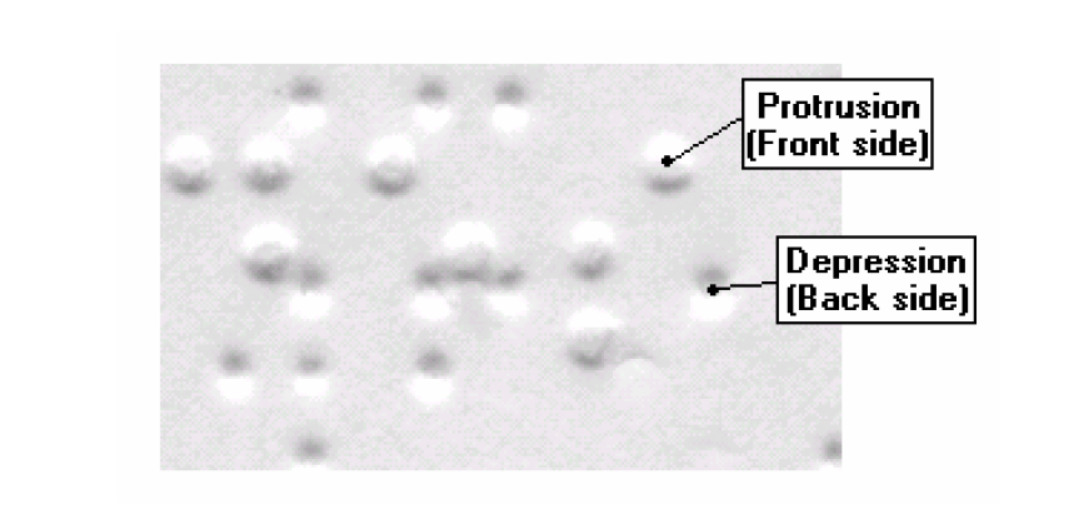
\includegraphics[width=1\linewidth]{front and backPNG.PNG}
\caption{front and back braille page}
\label{fig:acc}
\end{figure}

 Furthermore, the algorithm detects and corrects the document's skew angle using horizontal histogram analysis and calculation of mass centers. Notably, not all dots are detected using the overlapping process due to their small size or insufficient shadow overlap within the 4-pixel threshold. To address this, they introduce an adaptive algorithm to construct a Braille grid from the detected dots. 
 


In the grid construction phase, the adaptive algorithm starts by identifying columns aligned with the normalized distances between Braille dots. The initial stage focuses on grouping dots into vertical columns that conform to typical Braille dot spacing patterns. Subsequently, the algorithm adjusts the grid to accommodate variations in document layout, ensuring flexibility in column placement to handle slight deviations.
\begin{figure}[!ht]
\centering
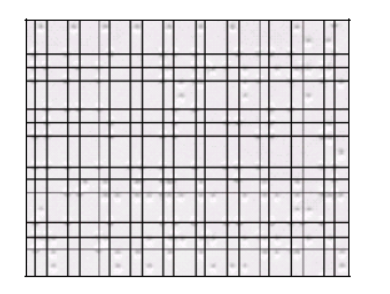
\includegraphics[]{grif.PNG}
\caption{the grid constructed for the detection}
\label{fig:acc}
\end{figure}


Similarly, the algorithm proceeds to establish rows aligned with Braille row patterns, completing the grid structure by integrating detected columns and rows. This flexible grid construction approach preserves the original document layout, enabling accurate representation of Braille positions without compromising format integrity.

Once the grid is established, the system employs dilation techniques to expand the search area around potential Braille dot positions. This step optimizes the system's efficiency by focusing detailed scrutiny on areas identified as potential Braille dot locations. Only positions that match the expected Braille dot criteria are validated, ensuring accurate detection while filtering out false detections that do not align with valid Braille dot locations.

Since the mentioned works essentially rely on snapping Braille points to the grid, they mostly work with images obtained with a scanner.

This methodical approach underscores the intelligence of the overall system, prioritizing time efficiency through targeted dot validation and ensuring robust detection of genuine Braille characters within scanned documents.

 
\paragraph{ W.D. Chamalee et al. [5] }
propose an algorithm designed to identify individual Braille characters on embossed printed paper using image processing techniques. Their method utilizes a stripping approach, which involves several key techniques such as dilation, standard distance ratios, and a vertical filling algorithm.

The algorithm is specifically tailored for embossed printed papers written in the Sinhalese language. It has been rigorously tested and demonstrates an impressive average accuracy of 99.2\%. This high accuracy underscores the effectiveness of their approach in reliably extracting Braille characters from printed documents, thereby enabling efficient and accurate optical Braille recognition.

\textbf{
\subsection{Using Convolutional Neural Networks (CNNs) for detecting Braille symbols}
}

\paragraph{In his paper on Optical Braille Recognition Using Object Detection CNN, Ilya G. Ovodov [6]}
 notes that while convolutional neural networks (CNNs) have significantly advanced image recognition in recent years, their application specifically to optical Braille recognition (OBR) is limited. He highlights sparse literature on the use of deep learning techniques, particularly fully connected neural networks (FCNs), in OBR. This observation underscores the nascent exploration of neural network applications in Braille recognition compared to their widespread adoption in general image recognition tasks.

Ovodov highlights the significant progress in computer vision, particularly in object detection, driven by Convolutional Neural Networks (CNNs) since their introduction by LeCun in 1989 and their explosion in popularity from 2012 onwards. Initially, CNN-based solutions for object detection involved separate processes for region proposal and object classification. Later advancements, such as Single Shot Multibox Detector (SSD) and You Only Look Once (YOLO), introduced the concept of one-stage detectors. These models generate a feature map where each point corresponds to a region of interest in the image. Anchors, predefined sizes for objects, are used to predict bounding box adjustments, object presence (confidence), and object class simultaneously. RetinaNet further improves upon these methods with the FocalLoss function, enhancing performance on challenging cases. Ovodov utilized these advanced CNN architectures for object detection in his research.

Ovodov's approach differs from traditional methods by directly detecting whole Braille symbols and recognizing them simultaneously using an object detection CNN. Each Braille character is assigned a class label ranging from 1 to 63 based on its composition of raised dots. The input images are scaled to 100 dpi, resulting in a resolution of 864x1150 pixels for standard A4 pages. Braille characters are identified with horizontal spacing of approximately 25 points and line spacing of about 40 points.

For implementation, Ovodov uses the RetinaNet CNN architecture with optimizations to handle the specific characteristics of optical Braille recognition. The architecture is simplified to reduce execution time, particularly focusing on non-maximum suppression (NMS) operations. A single "output to class + box subnet" is employed at the layer level with feature map cells of size 16x16 pixels, ensuring coverage of each Braille character. Only one anchor per grid cell, sized close to expected character dimensions, is utilized to further optimize performance.

To address potential overlap issues inherent in object detection, especially with small and uniformly sized objects like Braille characters, Ovodov lowers the Intersection over Union (IOU) threshold to 0.02 during NMS. This adjustment minimizes filtering errors and maintains high recognition quality despite detector imperfections.

These modifications significantly reduce computational time while preserving robust recognition capabilities tailored specifically for optical Braille recognition tasks.



\subsection{Recognition of Braille Symbols}

In optical Braille recognition, the recognition phase follows the detection of Braille symbols from scanned images. Unlike traditional approaches that separate stages for dot detection, grid restoration, and character combination, modern methods aim to directly recognize whole Braille symbols in a single step. This streamlined approach enhances efficiency and accuracy by leveraging advanced computational techniques tailored for Braille reading systems.

The recognition process involves assigning each detected Braille symbol a specific class label that corresponds to its Braille character representation. This classification allows for seamless translation into textual or auditory formats, ensuring accessibility for visually impaired individuals. The recognition algorithms analyze the spatial arrangement of dots within each symbol, interpreting their positions and configurations to determine the corresponding Braille character.

\paragraph{ Néstor Falcón et al. [1] }
describe a method where the final image, containing Braille dots represented as spots, undergoes thorough analysis for text segmentation into rows and characters. Utilizing the Braille grid previously constructed, which marks all positions of Braille dots, each character is then converted into a binary number based on the active dots present.

The segmentation process assigns a unique binary representation to each Braille character, leveraging a straightforward coding scheme that translates the presence of raised dots into '1's and absence into '0's. For example, the character 'r' in Braille, represented as '111010', illustrates this binary coding method where each '1' corresponds to an active dot ('mountain') on the Braille sheet.

This binary representation ensures language independence within the system, allowing for straightforward configuration adjustments to accommodate different alphabets or languages. Each character's binary number is then translated into its equivalent letter in standard text format, producing a final output in the form of a text file.

This approach not only simplifies the recognition and translation of Braille characters but also facilitates the seamless integration of optical Braille recognition systems into diverse linguistic environments.

\paragraph{In their paper "Deep Learning Strategy for Braille Character Recognition," Tasleem Kausar and colleagues [7]}
 propose a deep CNN model for Braille character recognition. The model comprises two main layers: feature extraction and classification. For feature extraction, they employ established deep CNN networks such as VGG16, ResNet50, InceptionV3, and DenseNet201, modifying the final layers with an IRB (Inverted Residual Block) module to enhance performance.

The architecture of DenseNet201, for instance, originally includes four dense blocks with transition layers. The researchers replace the last ten bottleneck layers in the final dense block with the IRB module. This module includes a 1x1 pointwise convolution before and after the depthwise convolution layer, effectively increasing the dimension of the output feature maps to enhance discriminative feature extraction.

By integrating these deep learning techniques, their model significantly improves the recognition accuracy of Braille characters, demonstrating the effectiveness of using advanced CNN architectures for optical Braille recognition.

\paragraph{In the article "Characterization of English Braille Patterns Using Automated Tools and RICA-Based Feature Extraction Methods," authors Sana Shokat, Rabia Riaz, Sanam Shahla Rizvi, Inayat Khan, and Anand [8]}
present a comprehensive comparison of different optical Braille recognition systems. They employ decision trees (DT), support vector machines (SVM), and k-nearest neighbors (KNN) combined with RICA- and PCA-based feature extraction techniques to predict Braille characters. Their research provides valuable insights into the effectiveness of various machine learning models and feature extraction methods in the recognition of Braille to English characters. The results are summarized in table 1 provided by the article. 

The highest performance was achieved with the RICA feature extraction method. DT achieved the highest accuracy (TA) and F1-Scores of 100\% for several characters, while KNN and SVM also showed excellent results with slightly lower scores. Using PCA, the accuracy was lower, with DT, SVM, and KNN achieving total accuracies of 70.02\%, 86.32\%, and 75.40\%, respectively. Random Forest with RICA, PCA, and Sequential models achieved accuracies of 80\%, 90.02\%, and 93.51\%, respectively.

Their research collected a new English Braille dataset using touchscreen devices. The authors used an Android application developed in their previous research to collect Braille English datasets. For visually impaired users, the application is less tiring and less complicated. Machine learning techniques such as SVM with polynomial kernels, KNN = 3, and Decision Trees with default parameters were combined with RICA- and PCA-based feature extraction methods for English alphabet recognition. For training and testing, the dataset was split into 70:30 and 80:20, respectively. Precision, Recall, F1-Score, and Accuracy were used as the evaluation metrics.  The SVM classifier outperformed all others, achieving an accuracy of 99.85\%. KNN and DT achieved 99.50\% and 99.79\% accuracy, respectively. For comparison, Random Forest with RICA, PCA, and Sequential methods were used, achieving accuracies of 90.01\% and 80\%, respectively.

By integrating these various recognition techniques, different Braille recognition systems achieve high accuracy in converting Braille dots into readable text, demonstrating the potential of advanced algorithms and deep learning in optical Braille recognition. \\

This comparison was very helpful in choosing the methods that we will be using in our project by avoiding the least accurate models and focusing on the most promising ones.
\newpage
\begin{table}[h!]
    \centering
    \begin{tabular}{|c|}
        \hline
        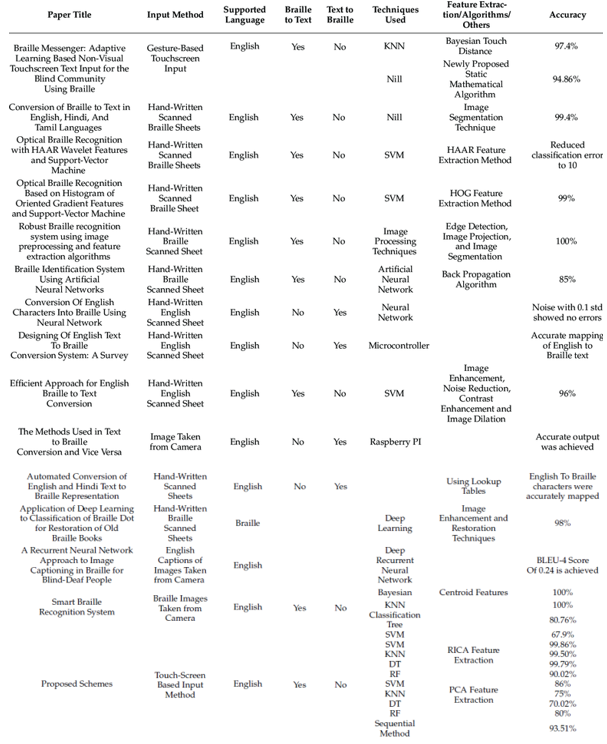
\includegraphics[width=\textwidth,height=22cm]{table 2.1.PNG} \\
        \hline
    \end{tabular}
    \caption{Comparative analysis of the feature Extraction/Detection techniques from previous studies }
    \label{tab: comparison}
\end{table}

\subsection{Text Correction Using Context}

One significant challenge in the translation of Braille to readable text is the issue of contextual accuracy. Misinterpretation of Braille dots can lead to incorrect characters, and without considering the context, words may be misinterpreted, particularly in languages with complex grammar. Additionally, Braille's specific formatting rules may not always translate seamlessly into text. Correcting these errors is crucial to ensure readability and accuracy. While standard spell checkers and grammar correction tools can address basic errors, they often fall short in understanding the context. This is where advanced methods, such as machine learning and contextual analysis, become essential. By leveraging neural networks and sequence-to-sequence models, it's possible to predict and correct errors based on the surrounding text. Contextual methods, such as n-grams and part-of-speech tagging, further enhance this process by providing a deeper understanding of sentence structure and word usage. However, even with sophisticated automated tools, human review remains invaluable for catching subtle errors. This highlights the need for a comprehensive approach to text correction that integrates automated tools with manual proofreading to ensure high-quality output. To delve deeper into the importance of context in spelling correction, we will discuss the findings from the paper titled "Spelling Correction Using Context" [9] which explores advanced techniques for enhancing text accuracy by focusing on the contextual relevance of words.

\paragraph{The system introduced by Elmi \& Evens}
 features an adaptive lexicon search and an intelligent filter to enhance processing speed. At its core, this approach leverages the interaction between a parser and a spelling corrector. The corrector proposes alternative spellings, which the parser then evaluates through syntactic and semantic checks within the dialogue, sentence, and phrase contexts.

Error detection is confined to isolated words. Once a misspelled word (S) is identified, the system follows a series of steps to find a suitable replacement. Initially, it selects a set of words from the lexicon for comparison. Then, it considers a configurable number of words similar to S as potential replacements. The final step involves using the sentence context to choose the best candidate, employing syntactic and semantic information along with phrase lookup to narrow down the options.

The system also allows users to set a limit on the number of errors. For a given limit (k), the program identifies all lexicon words that differ from the misspelled word by up to k mismatches, ensuring a comprehensive yet efficient correction process. This contextual approach significantly enhances the accuracy and reliability of the text correction, making it an invaluable tool for improving the readability of translated Braille text.\\

 

\subsection{Text to Speech}


 After successfully translating Braille text into readable text and ensuring accuracy through advanced correction techniques, the next crucial step in enabling accessibility for the visually impaired is converting this text into spoken language. This process, known as text-to-speech (TTS), plays a pivotal role in transforming written information into auditory output. Over the years, significant strides have been made in TTS technology, particularly through the pioneering work of researchers

\paragraph{Deep Voice, described in the research by Arık et al. [10]}
, represents an advanced neural network-based text-to-speech system designed for practical application. Unlike traditional methods that rely on complex feature engineering, Deep Voice utilizes deep neural networks across five core components. These include a model for phoneme boundary detection using connectionist temporal classification (CTC) loss, a grapheme-to-phoneme converter, models for predicting phoneme duration and fundamental frequency, and an efficient audio synthesis model inspired by WaveNet but with reduced complexity and faster training capabilities.

The use of neural networks in each component enhances the system's flexibility and simplifies its architecture compared to conventional text-to-speech systems. Importantly, the research demonstrates that the system can perform inference faster than real-time, showcasing optimized WaveNet inference kernels that achieve significant speed improvements on both CPU and GPU platforms. This innovation lays the groundwork for end-to-end neural speech synthesis, promising advancements in speech technology by leveraging deep learning techniques effectively.

The TTS system described in the Deep Voice paper comprises five integral components. First, the grapheme-to-phoneme model converts written text, represented in English characters, into phonemes using phonemic alphabet encoding like ARPABET. Subsequently, the segmentation model accurately identifies phoneme boundaries within voice datasets, pinpointing where each phoneme begins and ends in audio recordings. The phoneme duration model predicts the temporal length of each phoneme in an utterance, ensuring natural pacing and rhythm in synthesized speech. Meanwhile, the fundamental frequency model determines voicing and predicts fundamental frequency (F0) variations throughout phonemes, essential for generating lifelike intonation and pitch. Lastly, the audio synthesis model integrates outputs from the previous models to synthesize audio at a high sampling rate, aligning closely with the original text. During inference, text undergoes conversion into phonemes, followed by duration and F0 prediction, with these factors collectively conditioning the audio synthesis model to produce the final, coherent utterance.

\\
\paragraph{The Tacotron paper by Wang et al. [11]}
 introduces a groundbreaking approach towards achieving end-to-end speech synthesis directly from characters. Traditionally, such systems involve multiple stages including text analysis, acoustic modeling, and audio synthesis, each requiring specialized domain knowledge and often featuring rigid design choices. Tacotron, however, presents an innovative solution—a generative model that learns to synthesize speech from <text, audio> pairs starting from random initialization. The paper highlights several key techniques tailored for sequence-to-sequence learning, effectively addressing the complexities of this task. Notably, Tacotron achieves impressive results with a subjective mean opinion score of 3.82 on a 5-point scale for US English, surpassing the naturalness of existing parametric systems. Moreover, by generating speech at the frame level rather than sample-level autoregressive methods, Tacotron significantly enhances speed and efficiency in speech synthesis.

  As we conclude this comprehensive chapter, we have explored the intricate stages of optical Braille recognition from image preprocessing and filter application to precise Braille dot detection, symbol identification, and accurate symbol recognition. We have delved into the crucial aspect of text correction to ensure fidelity and accuracy in converting Braille symbols into readable text. Moreover, our journey has encompassed the transformative field of text-to-speech synthesis.

With these invaluable insights and methodologies at our disposal, our next ambition is to develop our own optical Braille recognition system. This system aims not only to convert images of Braille into correct textual representations but also to generate articulate speech, thereby enhancing accessibility for individuals with visual impairments. By leveraging advancements in image processing, machine learning, and speech synthesis techniques, we aspire to create a robust and inclusive solution that empowers users to access information independently and effectively. As we move forward into the next phase of development, we are dedicated to applying these lessons and exploring new possibilities to create solutions that are accessible to everyone.  


%********************************%
%***********SECTION 3************%
%********************************%
\newpage
\section{System Design and Architecture}
\setcounter{figure}{0}
\renewcommand{\thefigure}{3.\arabic{figure}}
In this chapter, we delve into the brief design and architecture of our system aimed at translating Braille pages to raw text and subsequently converting the text to speech. This chapter provides a comprehensive overview of the system's structure, components, and their interactions. By examining the system architecture, we gain insights into the design principles and considerations that guided the development process. This understanding is crucial for ensuring that the system operates efficiently, accurately, and reliably in translating Braille to accessible formats.




\subsection{Configurations}
\subsubsection{Printer Configuration and Paper Properties}
The specific paper type we used was provided by a specific printer to eliminate any distinct variation and ensure the persistence of high accuracy. 
\noindent \\Printer type: INDEX BRAILLE Everest-D V5\\
Printed page size: 23cm x 33cm\\
Dot size: 2mm\\
Distance between 2 dots in the same symbol:0.7mm\\
Distance between 2 rows: 3mm\\
Distance between 2 columns: 2mm\\
\begin{figure}[!ht]
\centering
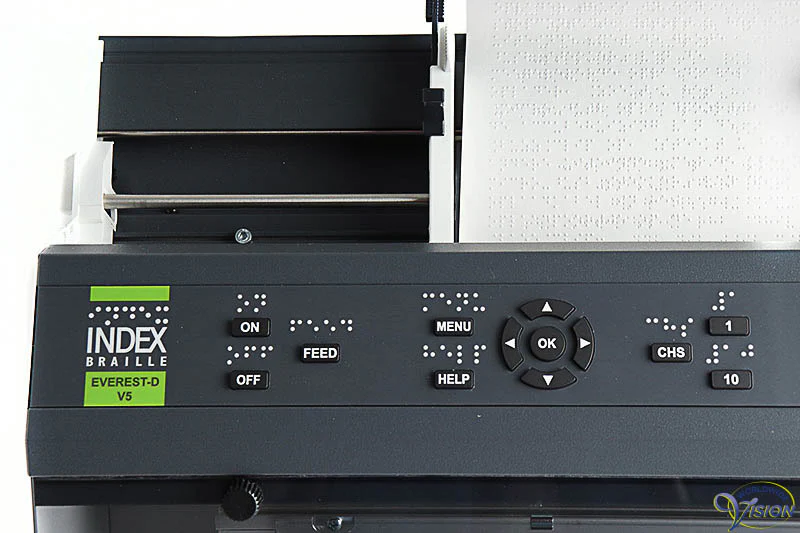
\includegraphics[width=0.4\linewidth]{printer.png}
\caption{INDEX BRAILLE Everest-D V5}
\label{fig:INDEX BRAILLE Everest-D V5}
\end{figure} \\

\subsubsection{Scanner configuration}
we used specific Scanner properties to remove any variations and ensure the persistence of high accuracy by supplying the preprocessing stage by the same properties of digitalized paper.\\

\noindent Source: Flatbed\\
Color format:	Grayscale\\
File type: JPG, PNG\\
Resolution (DPI): 100\\


    \clearpage
\subsection{Block Diagram }

\begin{figure}[!ht]
\centering
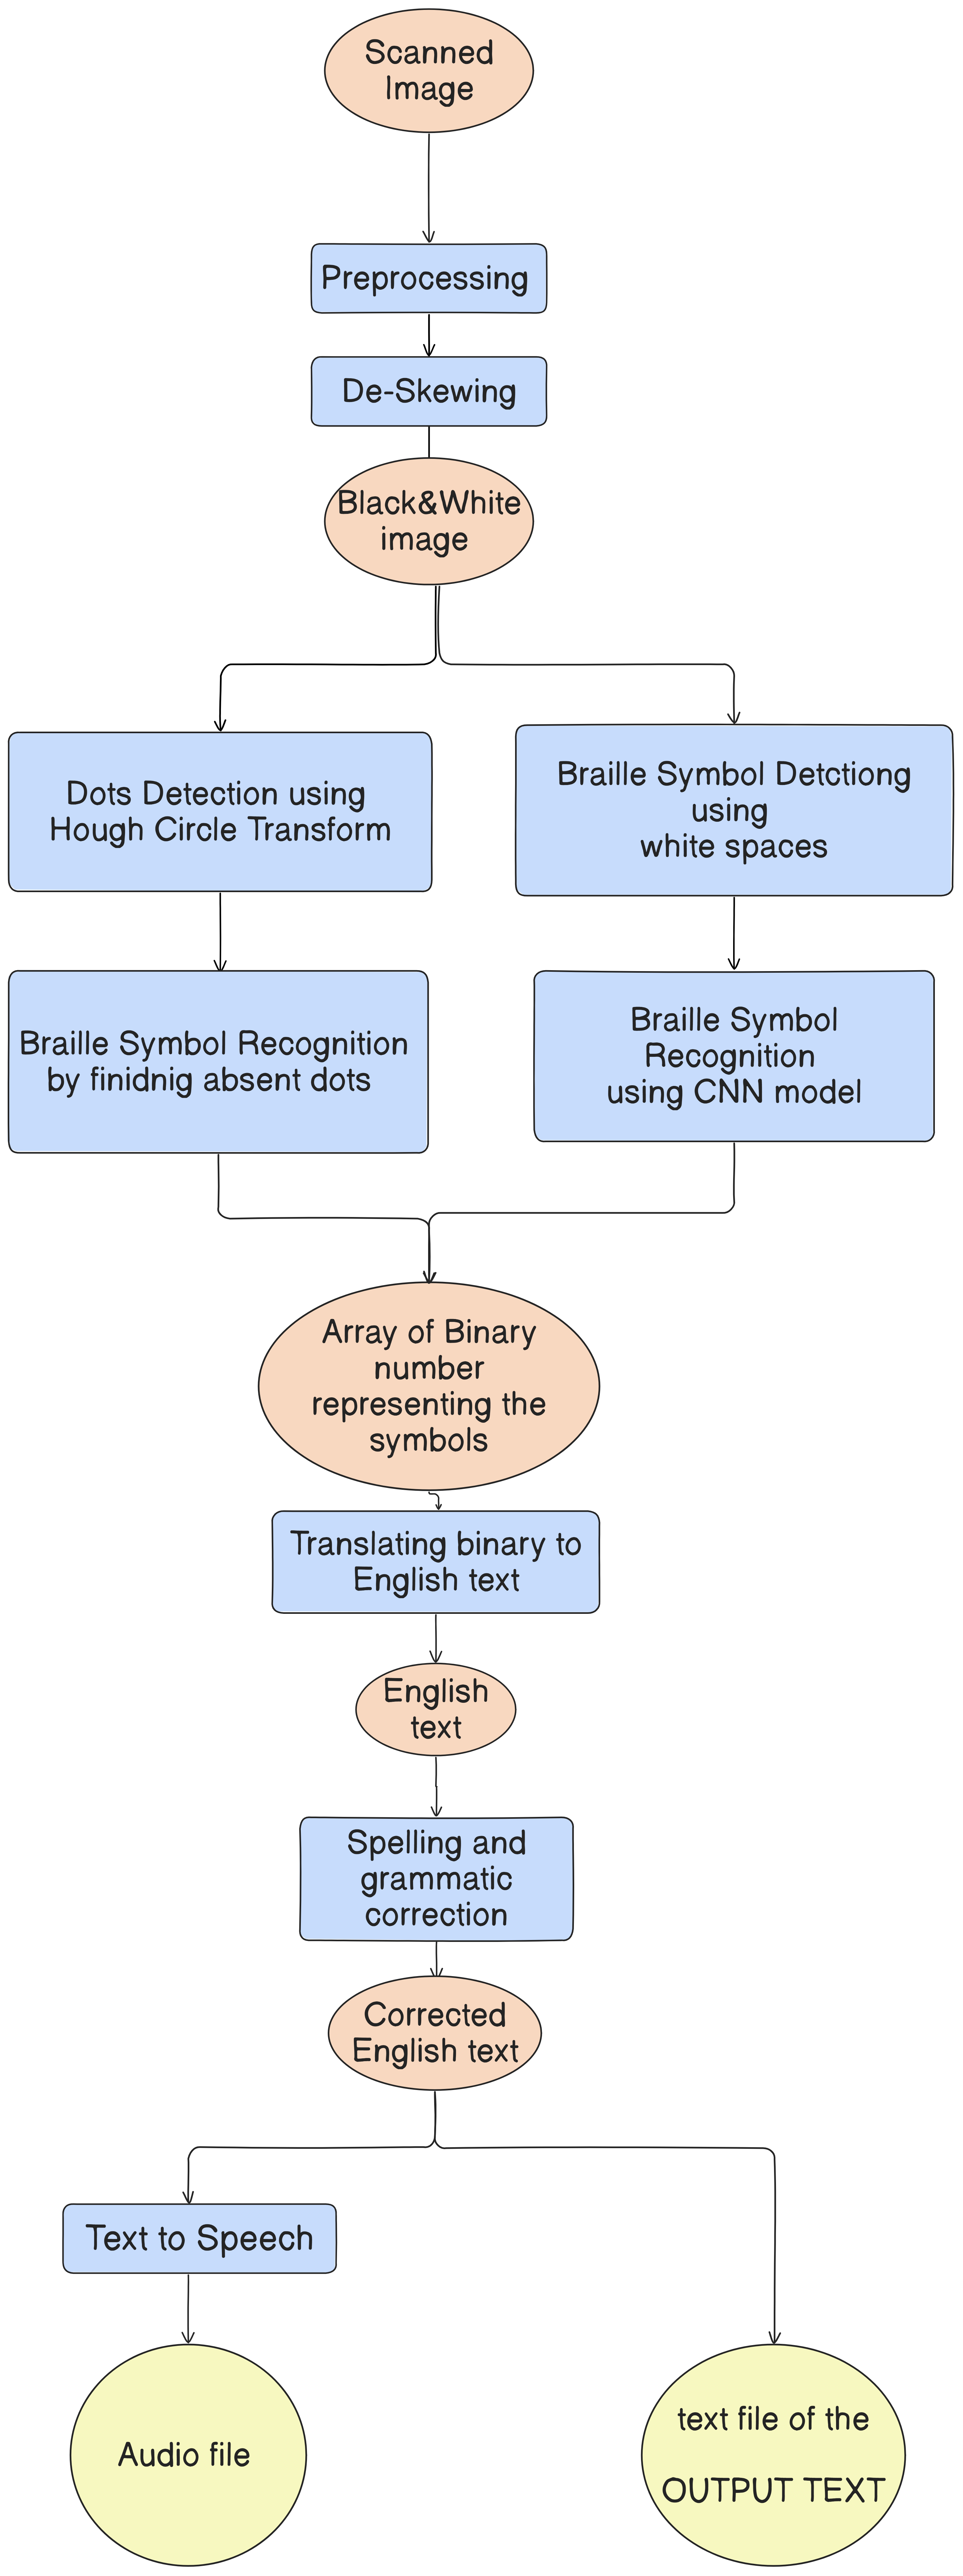
\includegraphics[width=0.55\linewidth]{BD.png}
\caption{Block Diagram}
\label{fig:Block Diagram}
\end{figure} \\

\newpage
The Block diagram, shown in Figure 3.2, illustrates the process of converting a scanned Braille image into readable and audible English text. Here's a step-by-step explanation:

\begin{enumerate}
    \item \textbf{Scanned Image}: The process begins with a scanned image of the Braille text using the scanner configuration mentioned above.

    \item \textbf{Preprocessing}: The scanned image undergoes several  filtering process which includes noise reduction and normalization. to prepare the image to be properly translated. this step reduces the complexity of  the next processes.

    \item \textbf{De-Skewing}: The image is de-skewed to correct any tilting that may have occurred during scanning, resulting in a properly aligned image.\\

\end{enumerate}
From this point, there are two paths for Braille symbol detection and recognition:\\

\paragraph{Path 1: Image Processing }
This path is illustrated as the right path of the block diagram shown in figure \ref{fig:Block Diagram}.

\begin{enumerate}
    \item \textbf{Dots Detection using Hough Circle Transform}: The Hough Circle Transform method is used to detect the centers of the circular shapes of Braille dots.

    \item \textbf{Braille Symbol Recognition by Finding Absent Dots}: A grid of all  possible symbols on a page is built. then the recognition process is done by comparing the grid to the detected Dots from the Hough circle transformation function. The presence or absence of dots in the recognized patterns decides  the Braille symbols.
\end{enumerate}

\paragraph{Path 2: CNN }
This path is illustrated as the left path of the block diagram shown in figure \ref{fig:Block Diagram}.

\begin{enumerate}
    \item \textbf{Braille Symbol Detection using White Spaces}: White spaces between the dots are used to detect the individual location of each Braille symbol.
    \item \textbf{Braille Symbol Recognition using CNN Model}: A Convolutional Neural Network (CNN) model is employed to recognize the Braille symbols from the detected patterns.\\
\end{enumerate}


After symbol recognition, both paths' output is a binary array of the braille symbols recognized as zeros and ones. The two paths then continue to the same post-recognition processes:

\begin{enumerate}

    \item \textbf{Translating Binary to English Text}: The binary numbers are translated into corresponding English text.
.
    \item \textbf{Spelling and Grammatical Correction}: The English text is corrected for any spelling and grammatical errors, resulting in corrected English text.
\end{enumerate}
Finally, the corrected English text can be output in two formats:

\begin{itemize}
    \item \textbf{Text to Speech}: The corrected English text is converted into an audio file.
    \item \textbf{Text File of the Output Text}: The corrected English text is saved as a text file.
\end{itemize}
This process allows for the conversion of Braille to both readable and audible formats, making the information accessible to a wider audience.

 


%********************************%
%***********SECTION 4************%
%********************************%
\newpage
\section{Preprocessing}
\setcounter{figure}{0}
\renewcommand{\thefigure}{4.\arabic{figure}}\\
\quad In this chapter, we will explore the preprocessing stage of our Braille
Translator system. We chose to implement a step-by-step approach,
gradually increasing complexity, rather than using all the filters from
the beginning. First, we will describe the challenges we encountered and
the phases we went through before discussing the filters used to address
these issues.

\hypertarget{development-phases}{%
\subsection{Development Phases}\label{development-phases}}\\
\quad Scanned papers often present various challenges, such as scanner noise, paper skewing, and damage due to being held too tightly. To address these issues effectively, we decided to begin our work with low complexity and gradually increase it, experimenting with different sources of noise at each step.\\
\hypertarget{Sample input 0}{%
\subsubsection{Sample input 0}\label{Sample input 0}}\\
\quad Recognizing the complexity of image processing tasks, we decided to
start with a flawless input initially. This approach
allowed us to test the functionality of our system before introducing
real-world application challenges.

\begin{figure}[h!]
     \centering
     \begin{subfigure}
         \centering
         
\includegraphics[width=\textwidth]{image1.png}
         \label{fig:Perfect braille image}
     \end{subfigure}
     \begin{subfigure}
         \centering
         
\includegraphics[width=\textwidth]{image2.png}
         \label{fig:Corresponding text}
     \end{subfigure}
        \caption{Braille writing using software tool}
        \label{fig:Braille writing using software tool}
\end{figure}\\
\quad We utilized a free online software tool that converts text to Braille characters, producing images with perfect dot sizing and coloring, and
free from noise, corruption, and rotation.\\

\hypertarget{Sample input 1}{%
\subsubsection{Sample input 1}\label{Sample input 1}}
\vspace{1em}\\
\quad During this phase, we faced one of the most significant challenges of
our project: Braille printing. Braille printers are rare, and although
we found a few, we could only gain limited access to one of them.\\

\quad We printed two pages with perfect specifications, free of noise and
errors. During this phase, we encountered some challenges and needed to
determine the optimal scanning method and quality to achieve the best
accuracy within a reasonable timeframe. We scanned the pages at 100 DPI,
concluding that this was a critical configuration point.\\

\quad In this phase, we sidestepped translation issues and treated the
program as separate modules. This approach allowed us to manage each
component individually before merging them back into the main program
branch in our workflow.\\
\clearpage
\begin{figure}[h!]
     \centering
         \centering
         
\includegraphics[width=.8\textwidth]{image5.jpg}
        \caption{Clear real braille samples}
        \label{fig:Clear real braille samples}
\end{figure}\\

\quad The primary challenge was to convert the scanned image into the clearest
possible version, like the ideal image used in phase 0. The filter stage
played a crucial role in this process. By applying specific filters such as Otsu's thresholding, GaussianBlur and medianBlur, we were able to enhance the clarity of the scanned image. These techniques will be discussed in detail later in this chapter.\\
\newpage
\hypertarget{Sample input 2}{%
\subsubsection{Sample input 2}\label{Sample input 2}}\\

\quad During this phase, we intentionally introduced various types of noise,
including light irregularities, corrupted pages, low-content pages, and
rotated pages. We successfully identified and categorized these issues,
resolving some while identifying others as critical points to avoid in
future processes.\\

\quad We will highlight the following critical points which we deem the
responsibility of the user:\\

\begin{enumerate}
\def\labelenumi{\arabic{enumi}.}
\item
  Users should refrain from gripping the paper too tightly to avoid
  damaging or distorting the dots.
\item
  Papers should be kept clean.
\item
  The scanner cover should be securely closed.
\end{enumerate}\\
\begin{figure}[h!]
    \centering
    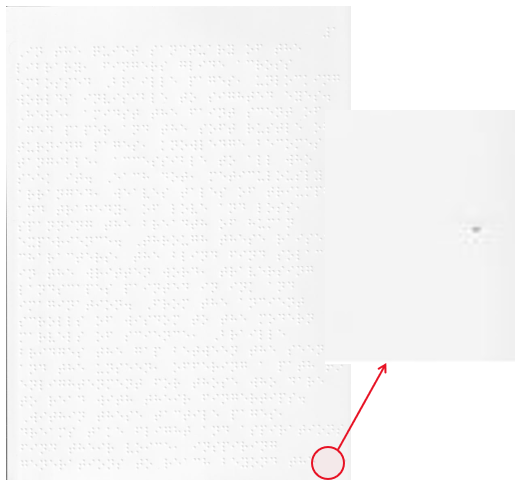
\includegraphics[width=.9\textwidth,height = 10cm]{A drop of dirt.png}
    \caption{A drop of dirt causes system failure}
    \label{fig:Clear real braille samples}
\end{figure}
\begin{figure}
    \centering
    
\includegraphics[width=.8\textwidth,height = 10cm]{held tight.png}
    \caption{Corrupted paper due to being held tight}
    \label{fig:Clear real braille samples}
\end{figure}\\
\begin{figure}[h!]
    \centering
    
\includegraphics[width=.9\textwidth,height = 10cm]{Low content.png}
    \caption{Low content pages contain light distribution irregularity}
    \label{fig:Clear real braille samples}
\end{figure}
\clearpage
\hypertarget{filters-and-opencv-methods-used}{%
\subsection{Filters and OpenCV methods
used}\label{filters-and-opencv-methods-used}}
\\
\quad Here is a block diagram illustrating the steps involved in our preprocessing system, which will be discussed in detail.\\
\begin{figure}[h!]
    \centering
    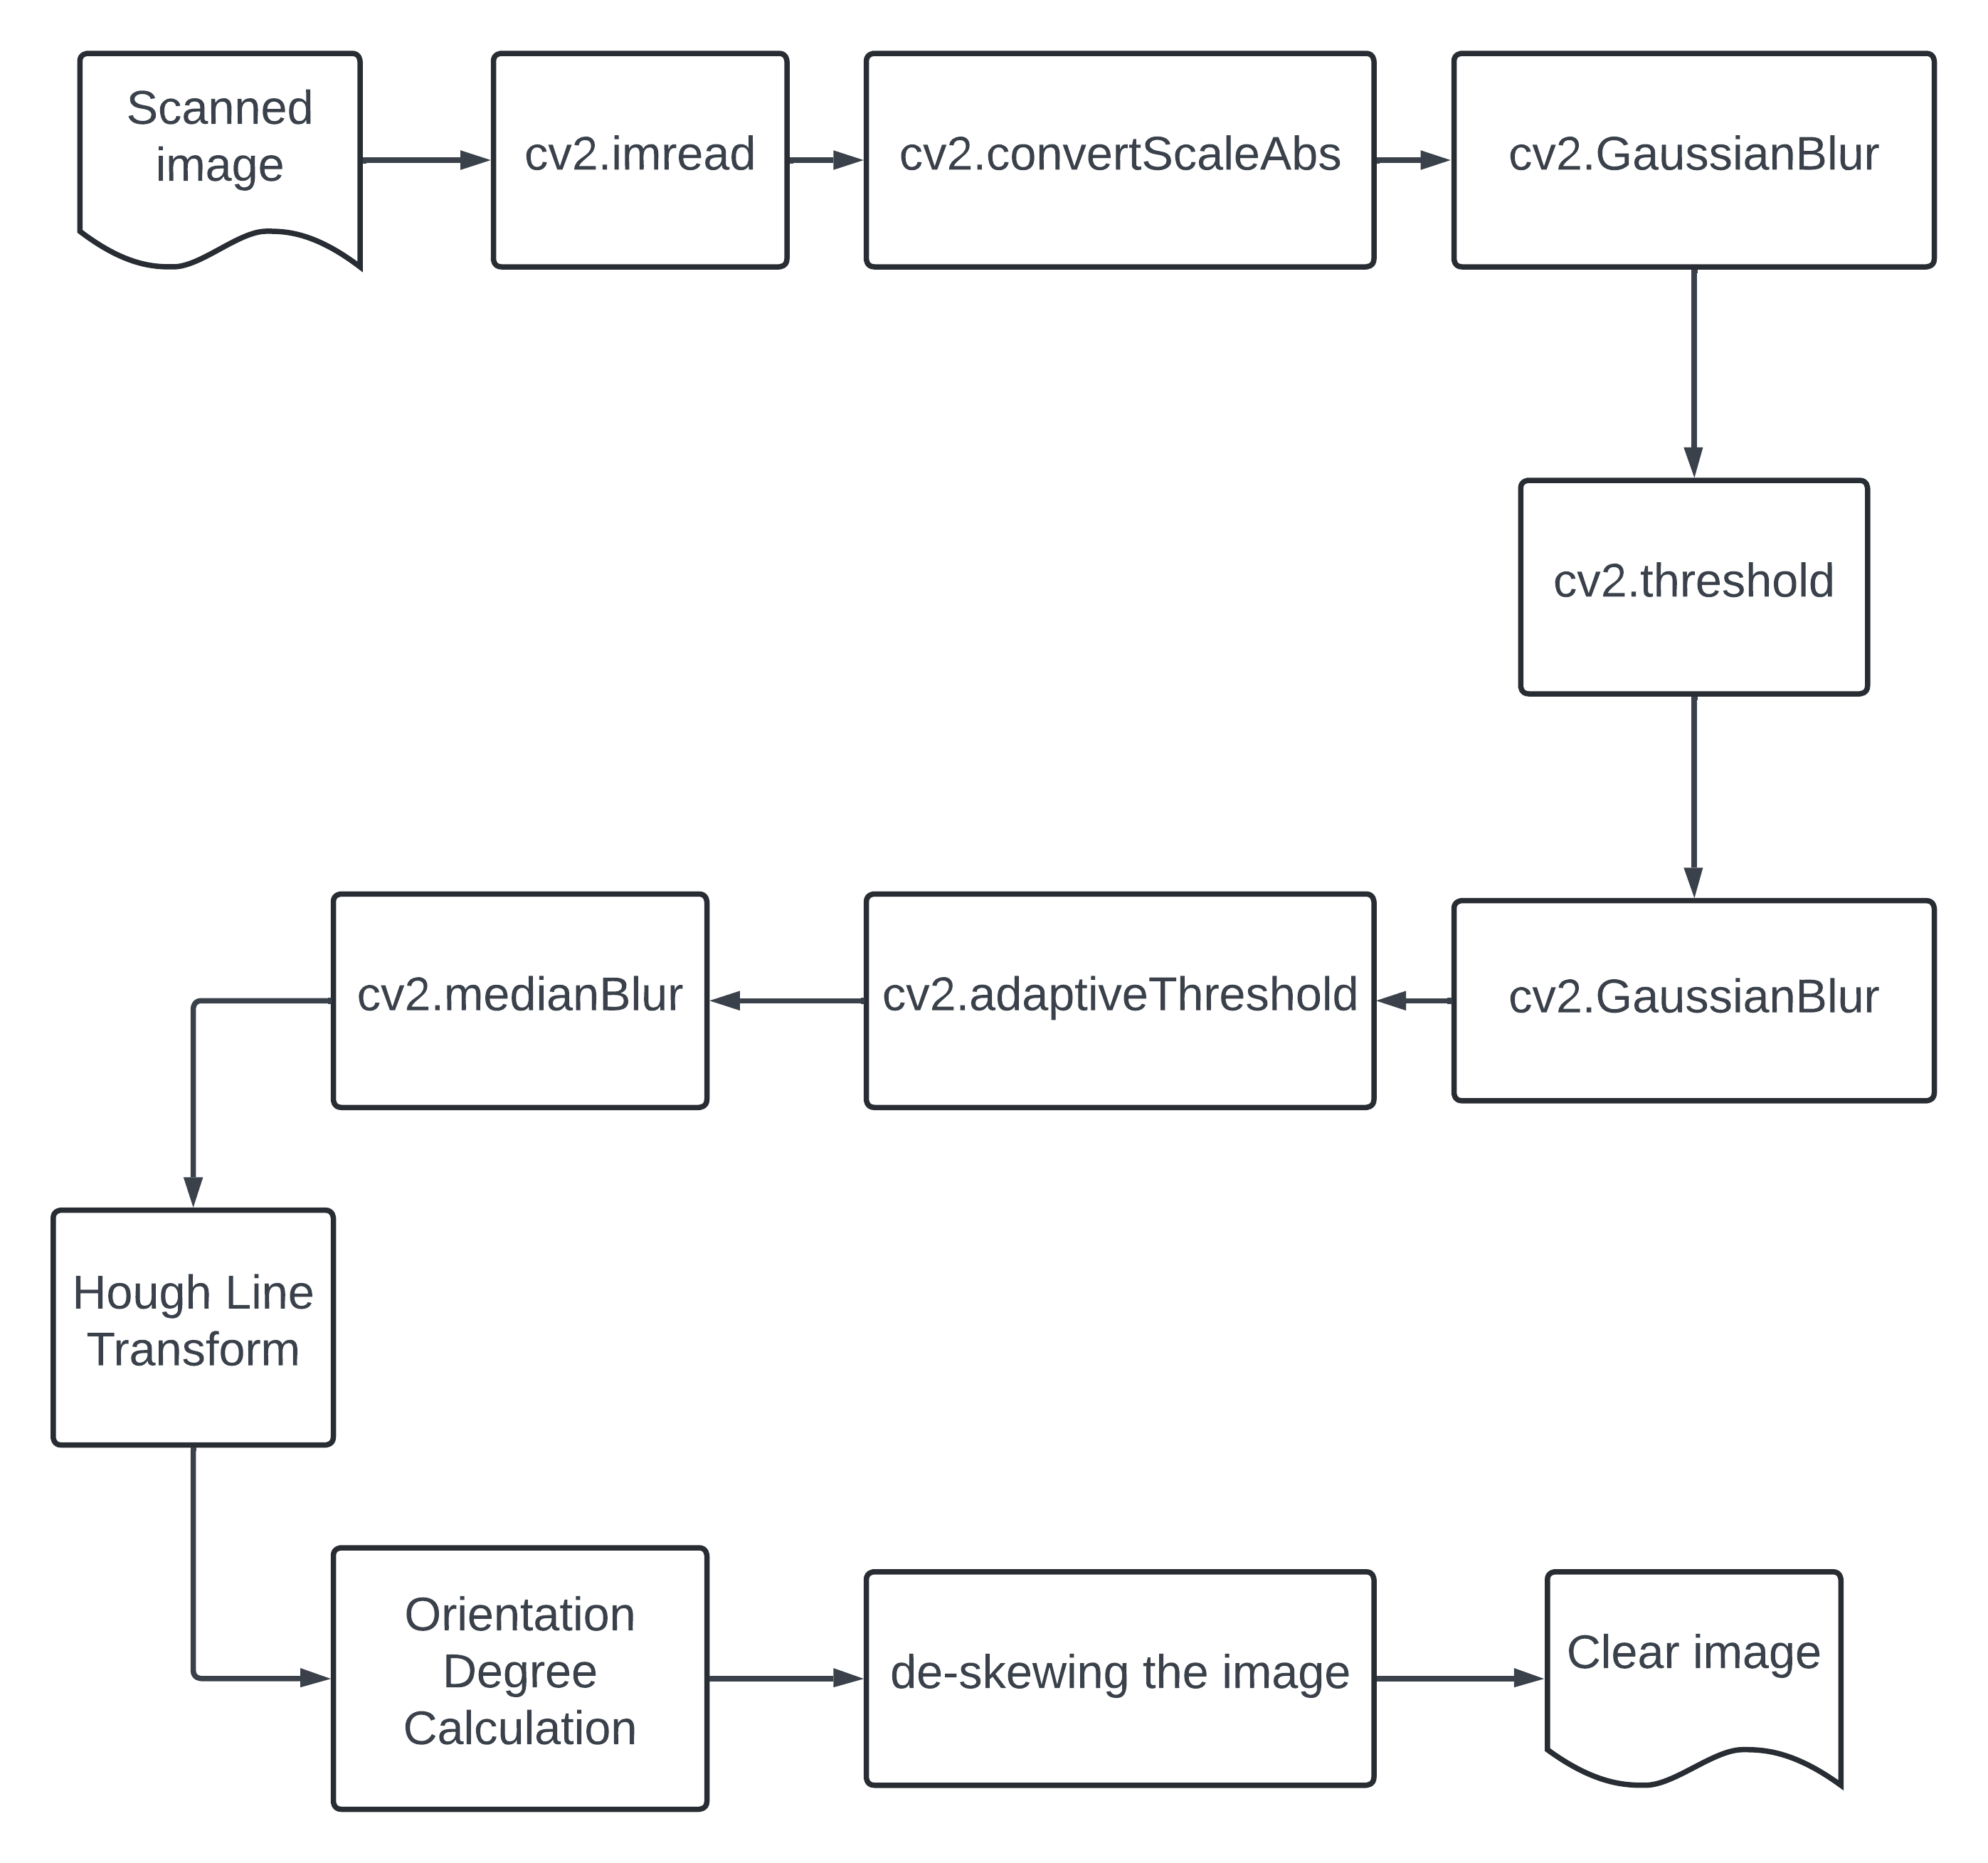
\includegraphics[width=.9\textwidth]{Preprocessing diagram.png}
    \caption{Preprocessing steps Diagram}
    \label{fig:Clear real braille samples}
\end{figure}
\newpage
\hypertarget{cv2.imread}{%
\subsubsection{cv2.imread}\label{cv2.imread}}

\begin{quote}
The method imread loads an image from the specified file and returns it.
\end{quote}\\

\begin{itemize}
\item
  The function determines the type of an image by the content, not by
  the file extension.
\item
  In the case of color images, the decoded images will have the channels
  stored in~\textbf{BGR}~order.
\item
  When using IMREAD\_GRAYSCALE, the codec\textquotesingle s internal
  grayscale conversion will be used, if available.
\item
  The dimensions of the scanned image using the scanner mentioned in the
  configuration section are (850 x 1169) at 100 DPI.
\end{itemize}\\


\begin{figure}[h!]
     \centering
        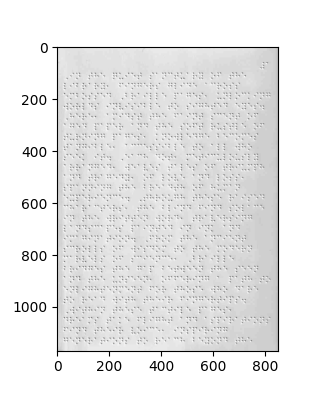
\includegraphics[width=0.8\textwidth,height=12cm]{image9.png}
        \caption{Scanned braille-written paper in general case}
        \label{fig:Scanned braille-written paper in general case}
\end{figure}\\


\hypertarget{cv2.convertscaleabs}{%
\subsubsection{cv2.convertScaleAbs}\label{cv2.convertscaleabs}}

\quad Scales, calculates absolute values, and converts the result to 8-bit.\\

\quad On each element of the input array, the function convertScaleAbs
performs three operations sequentially: scaling, taking an absolute
value, conversion to an unsigned 8-bit type:\\

\[dst(I) = saturate\backslash\text{\_}cast < uchar > (\left| src(I)*alpha + beta \right|)\]\\
\begin{itemize}
    \item \(\text{dst}(I)\): The destination pixel value at location \( I \).
    \item \(\text{src}(I)\): The source pixel value at location \( I \).
    \item \(\alpha\): A scaling factor applied to the source pixel values.
    \item \(\beta\): An added offset (brightness adjustment).
    \item \(\text{saturate\_cast}<\text{uchar}>\): Ensures the resulting value is clipped to the 8-bit range (0 to 255) and converted to an unsigned 8-bit type.
    \item \(| \ldots |\): Takes the absolute value of the expression inside.
\end{itemize}\\

\quad There are two tunable parameters which are alpha and beta, these
parameters have a huge impact in some special cases just as rotated
images and low content images.\\

\quad After a dedicated tuning session for these parameters to optimize the
mentioned special cases while maintaining the functionality in the
normal cases, it was proven that in our application alpha should be set
to (1.085) while beta performed just as required at a value of (-12).\\

\begin{figure}[h!]
     \centering
     \begin{subfigure}
         \centering
         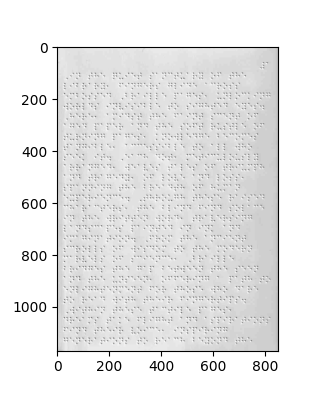
\includegraphics[width=.48\textwidth,height=8cm]{image9.png}
     \end{subfigure}
     \hfill
     \begin{subfigure}
         \centering
         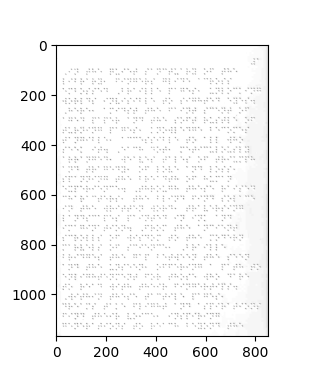
\includegraphics[width=.48\textwidth,height=8cm]{image11.png}
     \end{subfigure}
        \caption{Before and After applying convertscaleabs filter}
        \label{fig:Clear real braille samples}
\end{figure}\\

\newpage
\hypertarget{cv2.gaussianblur}{%
\subsubsection{cv2.GaussianBlur}\label{cv2.gaussianblur}}

Blurs an image using a Gaussian filter.\\

\quad The function convolves the source image with the specified Gaussian
kernel. In-place filtering is supported.\\

\quad We applied GaussianBlur twice due to its significant effect on noise
reduction. However, it must be used carefully to avoid erasing any
important data from the image. Here are some key functions of the
GaussianBlur filter in our application:\\

\begin{itemize}
\item
  \textbf{Noise Reduction}: The GaussianBlur filter effectively reduces
  noise by averaging the pixel values in a neighborhood defined by a
  Gaussian function. This helps in smoothing the image while preserving
  important structural details, making it easier to detect and recognize
  text or Braille dots.
\item
  \textbf{Edge Preservation}: Unlike other blurring techniques, the
  GaussianBlur filter maintains the integrity of edges, ensuring that
  the critical boundaries of characters or dots remain distinguishable.
  This is crucial for accurate feature extraction in subsequent
  processing stages.
\item
  \textbf{Preparation for Binarization}: GaussianBlur helps in creating
  a more uniform background, which is essential for effective
  binarization. A well-blurred image with uniform intensity levels
  facilitates better thresholding, resulting in a clearer distinction
  between the text/Braille dots and the background.
\item
  \textbf{Reducing Artifacts}: In images with varying light conditions,
  the GaussianBlur filter helps in reducing artifacts caused by shadows
  or uneven lighting. This normalization is important for maintaining
  consistency across different samples, ensuring reliable and repeatable
  results in the Braille translation process.
\end{itemize}\\
\begin{figure}[h!]
     \centering
     \begin{subfigure}
         \centering
         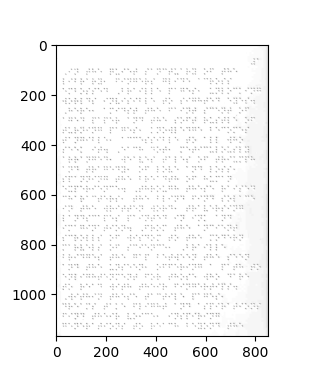
\includegraphics[width=.48\textwidth,height=8cm]{image11.png}
     \end{subfigure}
     \hfill
     \begin{subfigure}
         \centering
         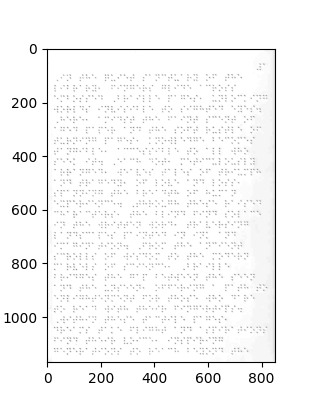
\includegraphics[width=.48\textwidth,height=8cm]{image13.png}
     \end{subfigure}
        \caption{Before and After applying the GaussianBlur filter}
        \label{fig:Clear real braille samples}
\end{figure}\\
\begin{quote}
Let's introduce the effect of the GaussianBlur filter on the previous image:
\end{quote}\\

\quad As shown in figure 4.7, GaussianBlur has a gentle effect on the edge
artifacts. It\textquotesingle s important to note
that at this stage, we used a mild GaussianBlur with a kernel of size 1
and a standard deviation of (1,1). These parameters will be adjusted
later to achieve a stronger blurring effect.\\
\newpage
\hypertarget{cv2.threshold}{%
\subsubsection{cv2.threshold}\label{cv2.threshold}}

\quad Applies a fixed-level threshold to each array element.\\

\quad The function applies fixed-level thresholding to a multiple-channel
array. The function is typically used to get a bi-level (binary) image
out of a grayscale image (compare~could be also used for this purpose)
or for removing a noise, that is, filtering out pixels with too small or
too large values. There are several types of thresholding supported by
the function. They are determined by type parameter.\\

\quad The special
values \textbf{THRESH\_OTSU} or \textbf{THRESH\_TRIANGLE}
be combined with one of various types of thresholding such as THRESH\_BIN and\\ THRESH\_BIN\_INV. In these cases, the function
determines the optimal threshold value using the Otsu\textquotesingle s
or Triangle algorithm and uses it instead of the specified threshold.\\

\quad \textbf{THRESH\_OTSU} is utilized in our application combined with\\ 
\textbf{THRESH\_BINARY} to simplify the task of converting the image
into a perfect black-and-white format. The significance of
Otsu\textquotesingle s thresholding lies in its ability to automatically
determine the optimal threshold value, enhancing the accuracy of the
binarization process. This method minimizes the variance within each
class of pixels, ensuring that the text stands out clearly against the
background, which is crucial for effective Braille translation. By using
Otsu\textquotesingle s thresholding, we enhance the reliability of our
preprocessing stage, making it easier to handle various image qualities
and conditions.\\

\quad This filter has 2 tunable parameters which are thresh (threshold value)
and maxval (maximum value to use with \textbf{THRESH\_BINARY} and \\
\textbf{THRESH\_BINARY\_INV} thresholding types)\\

\quad At this stage, we will obtain a clear image with low noise and high
contrast. We will reapply the GaussianBlur filter to further smooth the
image, maximizing the effectiveness of this step. This time, we will use
a stronger GaussianBlur with a variance of (3,3), as previously
mentioned. The results of each step in this stage are illustrated in the
following figures:  \\

\begin{figure}[h!]
     \centering
     \begin{subfigure}
         \centering
         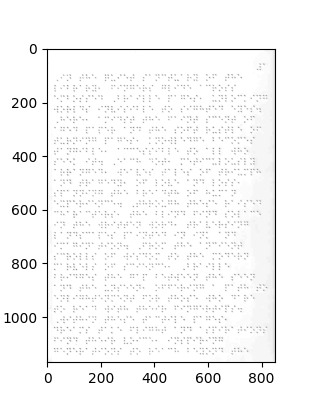
\includegraphics[width=.48\textwidth,height=8cm]{image13.png}
     \end{subfigure}
     \begin{subfigure}
         \centering
         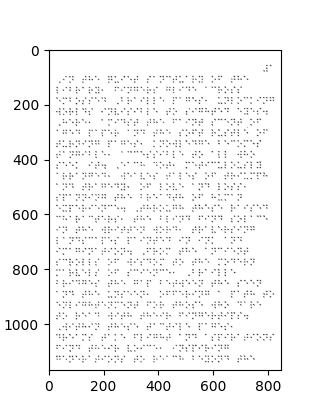
\includegraphics[width=.48\textwidth,height=8cm]{image15.png}
     \end{subfigure}
    \caption{Before and After Otsu's Threshold}
    \begin{subfigure}
    \centering
    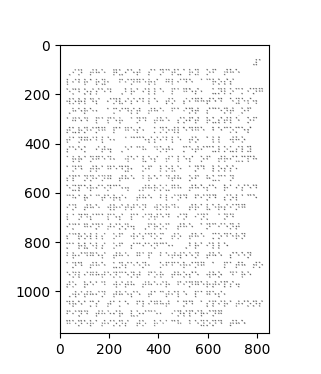
\includegraphics[width=.5\textwidth,height=8cm]{image16.png}
    \caption{After reapplying GaussianBlur}
    \label{fig:}
    \end{subfigure}
\end{figure}
\newpage
\hypertarget{cv2.adaptivethreshold}{%
\subsubsection{cv2.adaptiveThreshold}\label{cv2.adaptivethreshold}}\\

\quad In the previous section, we used a global value as threshold value. But
it may not be good in all the conditions where image has different
lighting conditions in different areas. In that case, we go for adaptive
thresholding. In this, the algorithm calculate the threshold for a small
regions of the image. So we get different thresholds for different
regions of the same image and it gives us better results for images with
varying illumination. So we can get the best case through this stage.\\

\quad The challenging aspect of this filter lies in fine-tuning its parameters
in conjunction with the previous stages to harness the benefits of
adaptive thresholding while avoiding its potential drawbacks in case of
inaccurate tuning. The key parameters are:\\

\begin{itemize}
\item
  \textbf{maxValue}: The non-zero value assigned to pixels that meet the
  condition.
\item
  \textbf{blockSize}: The size of the pixel neighborhood used to
  calculate the threshold value, typically an odd number like 3, 5, 7,
  and so on.
\item
  \textbf{C}: A constant subtracted from the mean or weighted mean,
  which can be positive, zero, or negative.
\end{itemize}\\

\quad For our purposes, these parameters were set to:\\

\begin{itemize}
\item
  \textbf{maxValue}: 255, since the background is pure white.
\item
  \textbf{blockSize}: 9
\item
  \textbf{C}: 21
\end{itemize}\\

\quad These values were determined through a trial-and-error tuning session.\\

\quad We can recognize from fig.4.12 that in this stage we have almost the
perfect image with high contrast, low noise which could be enough for
most cases but for some low content pages this stage is not enough so we
will go through the last and final filter in the next stage.\\

\begin{figure}[h!]
     \centering
     \begin{subfigure}
         \centering
         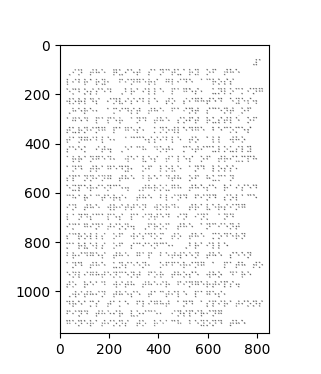
\includegraphics[width=.49\textwidth,height=8cm]{image16.png}
     \end{subfigure}
     \hfill
     \begin{subfigure}
         \centering
         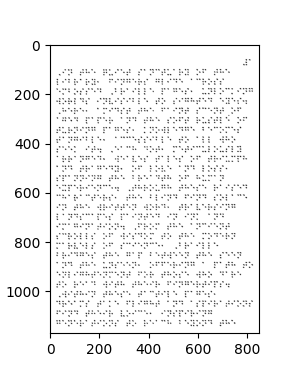
\includegraphics[width=.47\textwidth,height=8cm]{image19.png}
     \end{subfigure}
        \caption{Before and After applying AdaptiveThreshold}
        \label{fig:Clear real braille samples}
\end{figure}\\
\newpage
\hypertarget{cv2.medianblur}{%
\subsubsection{cv2.medianBlur}\label{cv2.medianBlur}}\\

\quad Median Blur is a powerful image processing filter that offers several
benefits, particularly in the context of noise reduction and edge
preservation:\\

\begin{itemize}
\item
  \textbf{Noise Reduction}: Median Blur is highly effective at reducing
  \textquotesingle salt-and-pepper\textquotesingle{} noise, a type of
  noise characterized by random bright and dark pixels scattered
  throughout the image.
\item
  \textbf{Edge Preservation}: Unlike other blurring techniques, Median
  Blur preserves edges while smoothing the image. which doesn\textquotesingle t blur sharp
  edges.
\item
  \textbf{Detail Retention}: It maintains the finer details in the
  image, making it useful for preprocessing steps where preserving
  important features is crucial.
\end{itemize}\\

\quad While Median Blur offers significant benefits, it also comes with
challenges:\\

\begin{itemize}
\item
  \textbf{Computational Intensity}: Median Blur can be computationally
  intensive, especially for large images or high kernel sizes, as it
  requires sorting the pixel values within the kernel for each pixel.
\item
  \textbf{Parameter Tuning}: Finding the optimal kernel size is critical
  and can be challenging. An inappropriate kernel size may either fail
  to remove noise effectively or excessively smooth the image, losing
  important details.
\end{itemize}\\

\begin{quote}
\quad The previous points show that the most important point to get the most
out of this filter is to perfectly identify the kernel size, the best
method to tune it is by starting with a small kernel and gradually
increase it to get the best accuracy with lowest computational power.\\

\begin{figure}[h!]
     \centering
     \begin{subfigure}
         \centering
         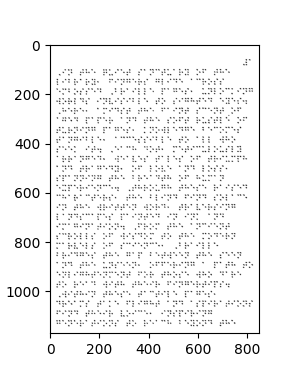
\includegraphics[width=.48\textwidth,height=8cm]{image19.png}
     \end{subfigure}
     \hfill
     \begin{subfigure}
         \centering
         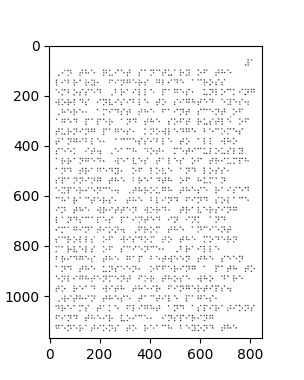
\includegraphics[width=.48\textwidth,height=8cm]{image21.png}
     \end{subfigure}
        \caption{Before and After applying the MedianBlur}
        \label{fig:Clear real braille samples}
\end{figure}
\newpage
\begin{figure}[h!]
     \centering
     \begin{subfigure}
         \centering
         
\includegraphics[width=.8\textwidth]{Before medianBlur.png}
     \end{subfigure}
     \hfill
     \begin{subfigure}
         \centering
         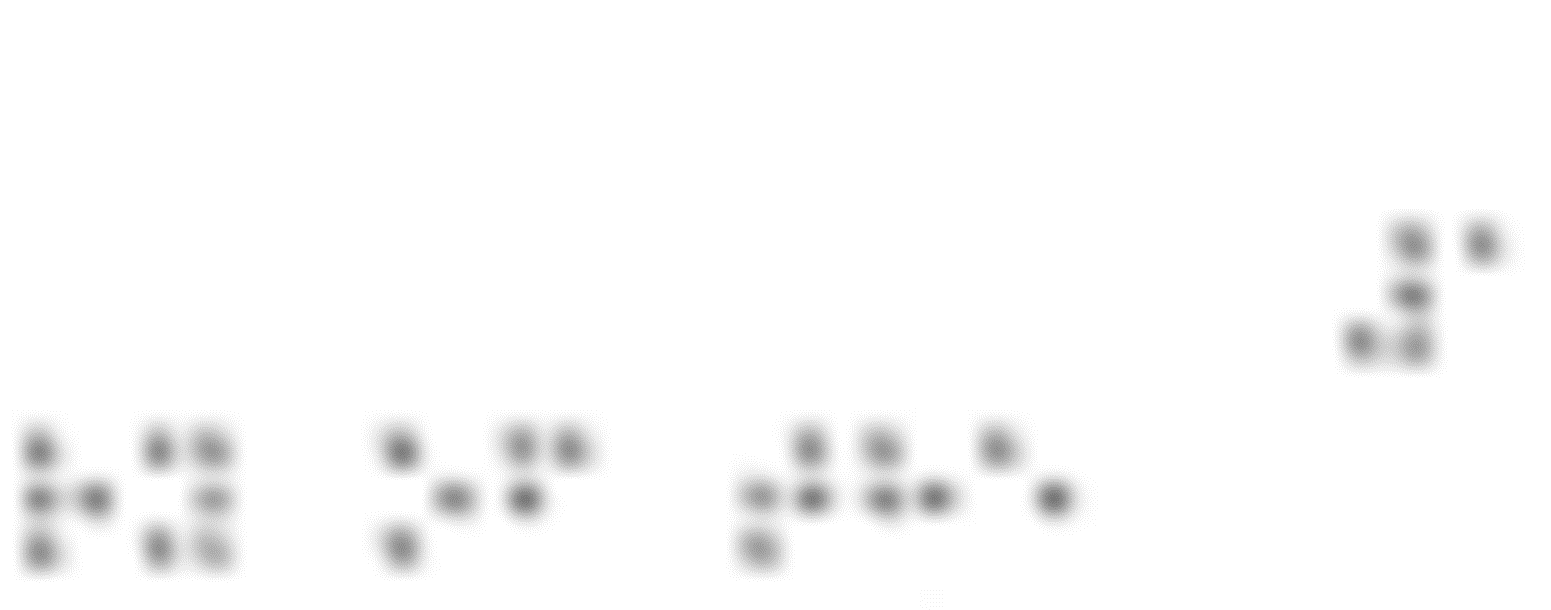
\includegraphics[width=.8\textwidth]{After medianBlur.png}
     \end{subfigure}
        \caption{zoomed look: Before and After applying the MedianBlur}
        \label{fig:Clear real braille samples}
\end{figure}\\
\quad in our case we only needed a small kernel of 3\textsuperscript{rd} degree
which has relatively low computational power.\\

\quad This concludes our preprocessing filters
section. We will now proceed to the next section, which focuses on
rotation correction.
\end{quote}\\

\newpage
\subsection{\textbf{Image Alignment and De-skewing } }\\
 The next challenge in preprocessing so then the image is ready for the detection step is De-skewing rotated images. This step is essential to enhance the accuracy of the next steps and to avoid over complicating the detection process.\\
\quad It is important to mention that the image must not be rotated with wide angles or else some of the dots will not scanned or partially scanned.\\
\quad To start facing the challenge we returned to the previous work by Isayed and Tahboub [4]. In their paper they have discussed many options to solve the skewing problem; linear regression method, standard deviation and Hough transform algorithm. We worked on both linear regression and Hough transform methods and found out that Hough transform method gives the most accurate results and the most generic for different examples and angles.\\
 \subsubsection{linear regression}
 \\
The idea in this method was to use the coordinates of the centers of the dot to find the angle of rotation. We used Hough circle transformation to find the coordinates, this is explained in chapter 5. We tried to find the angle using the linear equation Y=BX+A.
\begin{figure}[h!]
     \centering
        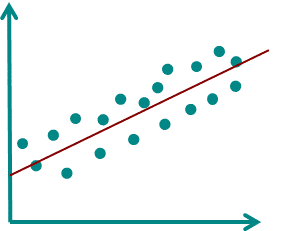
\includegraphics[width=0.3\textwidth]{Linear_regression_assumption_linearity.png}
        \caption{Scatter Plot with Linear Regression Line}
        \label{Scatter Plot with Linear Regression Line}
\end{figure}\\
 by calculating the slope of the straight line between two adjacent dots. The problem here is that the center detected by Hough circles method is not always the center of the dot. It might be shifted one or two pixels in any of the four directions. So, using only 2 adjacent dots is not effective.\\
 \quad We then started to work with 10 dots or more and try to find the best fitting line between the 10 dots and find the slope of this line.  for each 10 lines we find the slop and find the most repeated slope (mode of the slopes). from the slope we get the angle of rotation and use it to De-skew the image.
 The result of this method was not accurate having many problems:\\
 \begin{itemize}
    \item The slopes detected from each group of dots were not precise and gave different results.
    \item The angle chosen at the end was not accurate enough to continue to the next steps of the detection.
    \item This method was not generic for many Braille pages. It worked for one or two pages but then needed to be edited to be suitable for other pages.
\end{itemize}\\
\quad We tried to increase the number of dots in the group to find the best fitting line but that did not solve the problems we have. We also tried calculating the mean of the slopes instead of finding the mode but again all three problems were not solved. This pushed us to try other solutions.

\subsubsection{Hough line Transform method}
\\
The solution we tried next was to use the Hough transform to find the lines that connect the dots and find the angle of rotation. First we have to explain the how Hough transformation find the lines.\\

\textbf {Hough Line Transform}
\begin{enumerate}
    \item The Hough Line Transform is a transform used to detect straight lines.
    \item To apply the Transform, first an edge detection pre-processing is desirable.
\end{enumerate}\\

\textbf{How does it work?}

\begin{enumerate}
    \item A line in the image space can be expressed with two variables. For example:
    \begin{enumerate}
        \item In the Cartesian coordinate system: Parameters: (m, b).
        \item In the Polar coordinate system: Parameters: (r, $\theta$).
    \end{enumerate}
\end{enumerate}\\
\begin{figure}[h!]
     \centering
        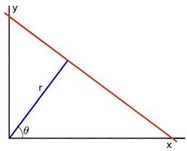
\includegraphics[width=0.6\textwidth]{Picture1.jpg}
        \caption{Representation of a Line in Cartesian and Polar Coordinate Systems}
        \label{Representation of a Line in Cartesian and Polar Coordinate Systems}
\end{figure}


For Hough Transforms, we will express lines in the Polar system. Hence, a line equation can be written as:\\
\[
y = \left(-\frac{\cos\theta}{\sin\theta}\right) x + \left(\frac{r}{\sin\theta}\right)
\]
Arranging the terms:
\[
r = x \cos\theta + y \sin\theta
\]

\begin{enumerate}
    \item In general, for each point \((x_0, y_0)\), we can define the family of lines that goes through that point as:
    \[
    r_\theta = x_0 \cdot \cos\theta + y_0 \cdot \sin\theta
    \]
    Meaning that each pair \((r_\theta, \theta)\) represents each line that passes by \((x_0, y_0)\).

    \clearpage
    \item If for a given \((x_0, y_0)\) we plot the family of lines that goes through it, we get a sinusoid. For instance, for \(x_0 = 8\) and \(y_0 = 6\) we get the following plot in figure  \ref{fig333} :

    \begin{figure}[h!]
     \centering
        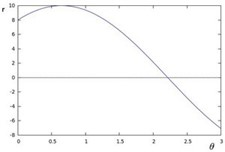
\includegraphics[width=0.6\textwidth]{Picture2.jpg}
        \caption{\(\theta - r\) plane for single selected point}
        \label{fig333}
    \end{figure}

    We consider only points such that \(r > 0\) and \(0 < \theta < 2\pi\).
    
    \item We can do the same operation above for all the points in an image. If the curves of two different points intersect in the plane \(\theta - r\), that means that both points belong to the same line. For instance, continuing with the example above and drawing the plot for two more points: \(x_1 = 4\), \(y_1 = 9\) and \(x_2 = 12\), \(y_2 = 3\), we get:
    \begin{figure}[h!]
     \centering
        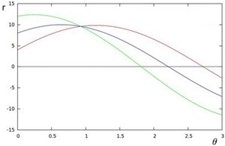
\includegraphics[width=0.6\textwidth]{Picture3.jpg}
        \caption{\(\theta - r\) plane for multiple selected point}
        \label{fig}
    \end{figure}
    The three plots intersect in one single point \((0.925, 9.6)\), these coordinates are the parameters \((\theta, r)\) of the line in which \((x_0, y_0)\), \((x_1, y_1)\), and \((x_2, y_2)\) lie.
    
    \item What does all the above mean? It means that, in general, a line can be detected by finding the number of intersections between curves. The more curves intersect, the more points lie on the line represented by that intersection. In general, we can define a threshold for the minimum number of intersections needed to detect a line.
    
    \item This is what the Hough Line Transform does. It keeps track of the intersections between curves of every point in the image. If the number of intersections is above some threshold, it declares it as a line with the parameters \((\theta, r_\theta)\) of the intersection point.
\end{enumerate}\\

\textbf{Standard and Probabilistic Hough Line Transform\\}

OpenCV implements two kinds of Hough Line Transforms:\\

\textbf{The Standard Hough Transform}
\begin{itemize}
    \item It consists of pretty much what we just explained in the previous section. It gives as a result a vector of pairs \((\theta, r_\theta)\).
    \item In OpenCV, it is implemented with the function \texttt{HoughLines()}.
\end{itemize}\\

\textbf{The Probabilistic Hough Line Transform}
\begin{itemize}
    \item A more efficient implementation of the Hough Line Transform. It gives as output the extremes of the detected lines \((x_0, y_0, x_1, y_1)\).
    \item In OpenCV, it is implemented with the function \texttt{HoughLinesP()}.
\end{itemize}

\subsubsection{Applying the Hough Transformation for Line Detection and page De-Skewing}
\quad To use the Hough transformation, we pass the scanned image through filtering process, discussed earlier in this chapter. The resulted black \& white image, shown previously in figure 4.13, is passed through edge detection filter that uses canny algorithm, which is going to be explained in details in chapter 5.  \\
\quad The next step is the Hough transformation. We used the OpenCV function HoughLinesP(). this function takes an input image and pass an array of lines as an output. The function also takes other parameters like minimum line length which was 90 pixels in our implementation and the maximum line gap, 200 pixels. These values were reached by trail to reach the best results.\\

\quad For illustration the lines are drawn on the input image to show the output of the function. Figure 4.19 compares between the input image and the output of the HoughLinesP() function. \\

The precision of the lines can be observed in Figure 4.19 (b). Most of the lines extracted are horizontal with a small angle to the x-axis. There are also some vertical lines with the same angle but to the y-axis. The diagonal lines are to be ignored as they are considered noise. \\

Some pages will have more vertical lines than horizontal lines so we rotate all the angles between 80 and 100 degrees with the horizontal axis by 90 degrees to add these lines to our next steps. We also removed any diagonal lines to avoid their effect while calculating the angle of rotation. We then calculate the mean of all the angles to find the angle of rotation. For example, the angle of rotation in figure 4.19 is -0.99469 degrees. \\



\begin{figure}[H]
\centering
\subfloat[rotated scanned image]{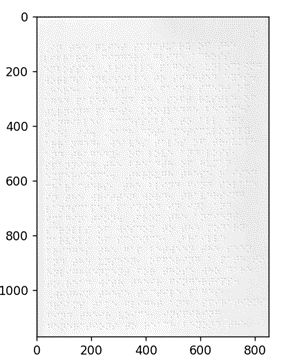
\includegraphics[width=0.6\linewidth]{Picture4.png}}\hfill
\subfloat[lines on the rotated page]{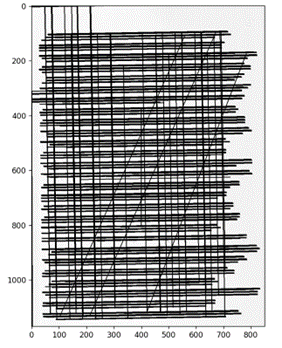
\includegraphics[width=0.6\linewidth]{Picture5.png}}\\
\caption{Using Hough line transform on rotated image}
\label{fig:num1235}
\end{figure}

\newpage


 The next step is to calculate the angle between the horizontal x-axis and the lines. That is easily done by finding two points of each line and calculate the slope as arctan the angle. \\



The angle of rotation is used to rotate the image using built in functions in python. The output of the rotation function is shown in figure 4.20. A border is added after rotation. We have chosen white border to blend with the background of the processed image. The additional border adds noise in the middle between the border and the image. This noise can be detected by the detection process coming next. So we have to remove that part even it is as small as in the figure. This is done by finely cropping the edges of the image to remove the noise without affecting any of the dots. The final image after cropping that can be used in the next steps of our project is shown in figure 4.20 (b). \\

\begin{figure}[h!]
     \centering
     \begin{subfigure}
         \centering
         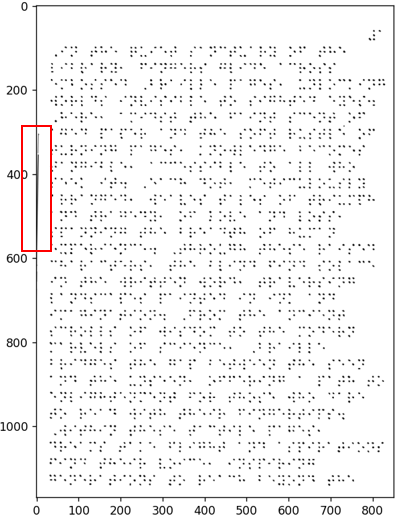
\includegraphics[width=.45\textwidth]{Picture6.png}
     \end{subfigure}
     \hfill
     \begin{subfigure}
         \centering
         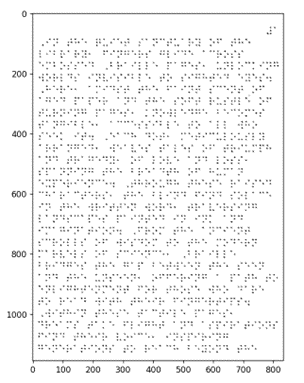
\includegraphics[width=.478\textwidth]{Picture7.png}
     \end{subfigure}
        \caption{(a) image after rotation \quad (b) image after cropping the edges }
        \label{fig:orientation}
\end{figure}
\textbf{\\ Discussion \\}
\\
\quad The rotation algorithm we used showed great results and the rotated images were almost the same accuracy as an upright scanned image. The system was tested with images rotated with angles between -2 and 2 degrees. the system was able to calculate the angle with accuracy to the fifth decimal point of a degree. \\
\quad One of the problems of rotated image is that the dots fades slightly compared to the upright image due to the kernel used in the filters. The tuning of the filters was done to be affective with all angles in the range we tested. However, the faded dots can affect the detection result but as our results show it does not exceed 1\% of the symbols and all these errors is detected and corrected by the correction part in our project.   \\


%********************************%
%***********SECTION 5************%
%********************************%
\newpage
\section{Detection and Recognition Using Image Processing}
\setcounter{figure}{0}
\renewcommand{\thefigure}{5.\arabic{figure}}

In this Chapter, we will go through the full process of turning a single sided Braille page loaded with multiple characters and full of Braille dots that has been preprocessed into multiple arrays of zeros and ones representing all of the symbols in the page. This page has already been filtered and adjusted to be correctly oriented. 

Before going through the details, let's discuss the keywords used in this chapter. The term "Detection" refers to the process of locating each braille symbols in a page. Producing an output array that contains all of the locations of the dots in the page. On the other hand, the term "Recognition" refers to the process of identification of each symbol as a combination of 6 dots.

It is important before explaining the algorithm used for detection to mention the restriction to the input page. For simplicity we assumed that the input page would have multiple lines - full of symbols - and not just a line or two. This is to ensure a maximum accuracy in the detection process. The explanation for this restriction is to be discussed later in this chapter.
\subsection{Detection}
In this section we will discuss the methods used to extract locations of the dots in our Braille page. The two methods are mainly \textit{Canny Edge Detection} and \textit{Hough Circle Detection} which are complementary to each other.
\subsubsection{Edge Detection with Canny Algorithm}
Canny edge detection is a technique designed to extract essential structural details from various visual objects while significantly reducing the data that needs processing. It's widely used in different computer vision applications due to its effectiveness in meeting the general requirements for edge detection across diverse systems. These requirements include:
\begin{enumerate}
        \item Detecting edges with a low error rate to ensure that as many edges as possible in the image are accurately identified.
        \item Precisely localizing the detected edge points to the center of the edges.
        \item Ensuring that each edge in the image is marked only once and minimizing the impact of image noise to avoid false edges.
\end{enumerate}


To meet these criteria, Canny employed the calculus of variations, a technique that finds the function optimizing a given functional. The optimal function in the Canny detector is represented by the sum of four exponential terms but can be approximated by the first derivative of a Gaussian.

The Canny edge detection algorithm is one of the most well-defined methods for edge detection, known for its reliability and effectiveness. Due to its optimality in meeting the three key criteria and the simplicity of its implementation, it has become a popular choice for edge detection.

The Canny edge detection process involves five main steps:

\begin{enumerate}
        \item Apply a Gaussian filter to smooth the image and reduce noise. Fig.\ref{fig:num1}(b)
        \item Calculate the intensity gradients of the image. Fig.\ref{fig:num1}(c)
        \item Use gradient magnitude thresholding or lower bound cut-off suppression to eliminate spurious edge detection responses. Fig.\ref{fig:num1}(d)
        \item Apply a double threshold to identify potential edges. Fig.\ref{fig:num1}(e)
        \item Use edge tracking by hysteresis to finalize edge detection by suppressing weak edges that are not connected to strong edges. Fig.\ref{fig:num1}(f)
\end{enumerate}

\begin{figure}[H]
\centering
\subfloat[Original Image]{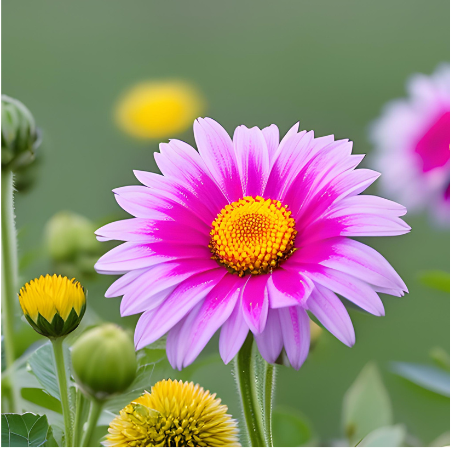
\includegraphics[width=0.45\linewidth]{Canny/0.png}}\hfill
\subfloat[Image after greyscale and noise reduction]{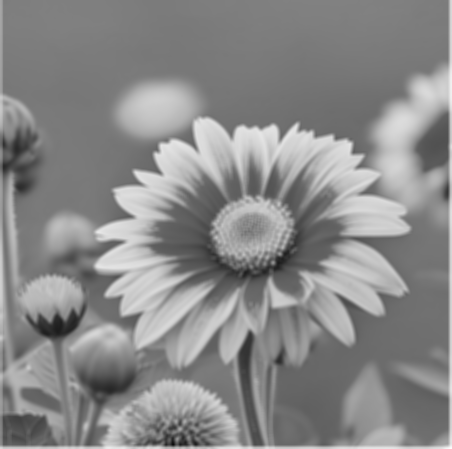
\includegraphics[width=0.45\linewidth]{Canny/1.png}}\\
\subfloat[After gradient calculation]{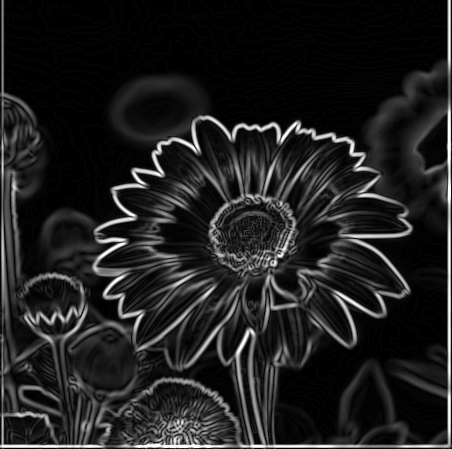
\includegraphics[width=0.45\linewidth]{Canny/2.png}}\hfill
\subfloat[After non-maximum suppression]{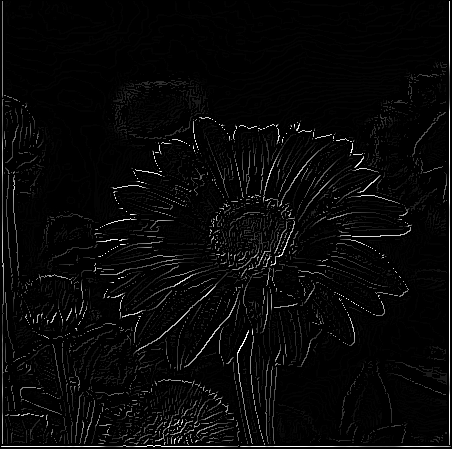
\includegraphics[width=0.45\linewidth]{Canny/3.png}}\\
\subfloat[Strong edges after double thresholding]{
\includegraphics[width=0.45\linewidth]{Canny/4.png}}\hfill
\subfloat[Final edge tracking]{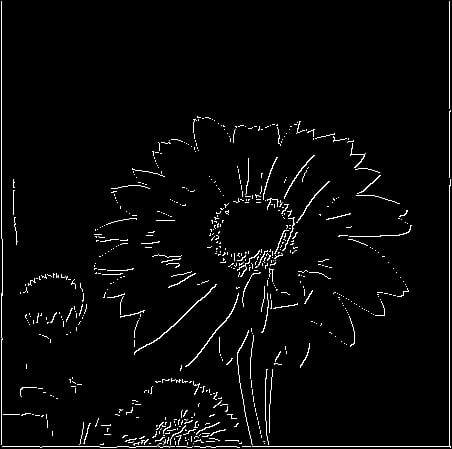
\includegraphics[width=0.45\linewidth]{Canny/5.jpeg}}
\caption{Canny Edge Detection Process}
\label{fig:num1}
\end{figure}
\clearpage

While dealing with a loaded page of Braille symbols, the process is just the same as mentioned above. All the manipulation is done through adjusting the parameters and resolution of the filters until getting the perfect output. Fig.5.2(b) shows the single sided Braille page after being processed with canny algorithm.
\begin{figure}[H]
    \centering
    \subfloat[Original Page (After Preprocessing)]{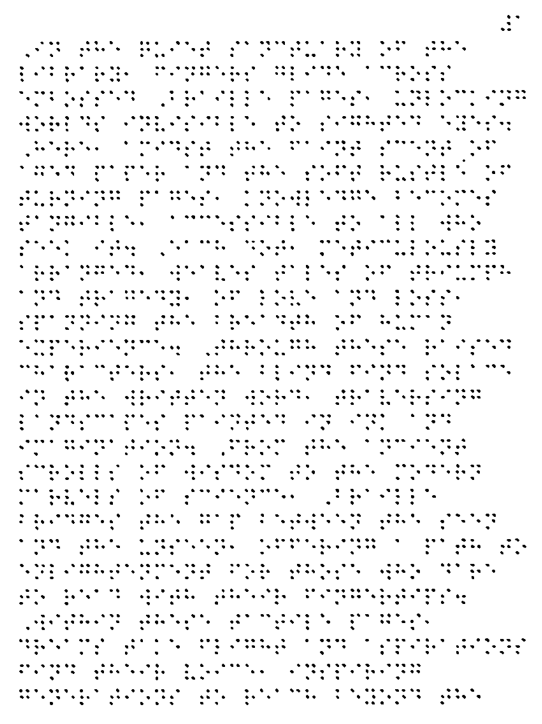
\includegraphics[width=0.5\linewidth]{Canny/filtered.png}}\hfill
    \subfloat[Detected Edges]{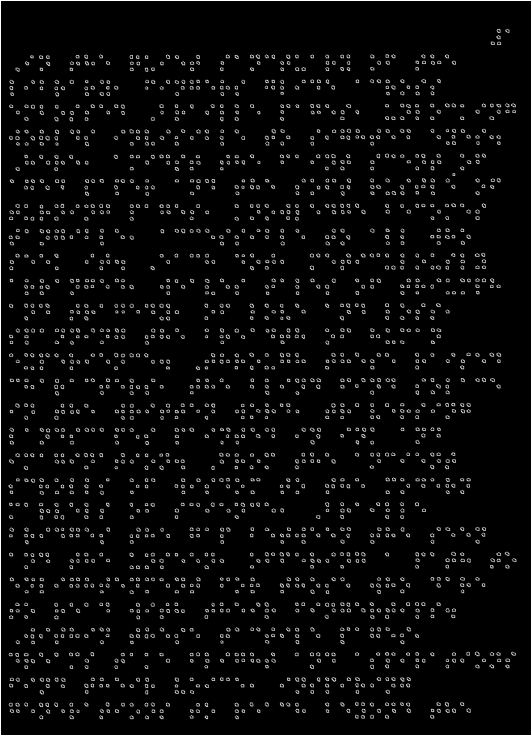
\includegraphics[width=0.5\linewidth]{Canny/Edges.png}}\\
    \caption{Canny Process Applied to the filtered \& upright Braille page}
    \label{fig:num2}
\end{figure}




\subsubsection{Circle Detection with Hough Transform}

\textbf{\textit{Theory of Hough Circle Transform}}

The Hough Circle Transform is a feature extraction technique used in image processing for detecting circles in an image. This method is an extension of the Hough Transform, which is widely used for detecting various shapes, especially lines. The classical Hough Transform for line detection involves mapping points from the image space to the parameter space, where lines in the image space correspond to points in the parameter space. Similarly, in the Hough Circle Transform, the goal is to identify circular shapes by mapping image space coordinates to the parameter space defined by the circle's parameters: center coordinates \((x_{center}, y_{center})\) and radius \(r\).

Mathematically, a circle can be described by the equation:
\begin{equation}
(x - x_{center})^2 + (y - y_{center})^2 = r^2
\end{equation}

where \((x_{center}, y_{center})\) represents the center of the circle and \(r\) its radius. To detect circles, the algorithm uses a parameter space that is three-dimensional, with dimensions corresponding to the circle's center coordinates and radius. For each edge point \((x, y)\) in the image, the possible circles passing through that point are determined, and an accumulator array in the parameter space is incremented accordingly. The peaks in this accumulator array indicate the parameters of the circles present in the image.

\textbf{\textit{Differences from Hough Gradient Method}}

The Hough Gradient Method, also known as the Hough Gradient Transform, is a more efficient variant of the classical Hough Circle Transform specifically designed for circle detection. While the traditional Hough Circle Transform involves a computationally expensive three-dimensional search for circle parameters, the Hough Gradient Method incorporates edge detection and gradient information to streamline this process.

The Hough Gradient Method reduces the computational complexity by taking advantage of the gradients of edge points. Here’s how it works:
\begin{enumerate}
        \item \textbf{Edge Detection:} Initially, an edge detection algorithm like Canny Edge Detector - discussed in section 5.1.1 - is applied to the image to find the edge points.
        \item \textbf{Gradient Computation:} For each edge point, the gradient direction is computed. The gradient direction indicates the direction of the center of the circle for that edge point.
        \item \textbf{Voting in Accumulator Space:} Using the gradient information, the algorithm only votes for circle centers along the gradient direction, significantly reducing the number of potential centers compared to the traditional method that votes in all directions.
\end{enumerate}


This method significantly enhances efficiency because it narrows down the potential circle centers by leveraging the directional information from gradients. Consequently, the Hough Gradient Method requires fewer computational resources and provides more accurate circle detection by reducing false positives.

Applying the Hough Gradient Method to the Braille page that has gone through the process of edge detection not only required low computational power, but also showed great results as it successfully detected all of the dots locations in the page. Figure \ref{fig:num3}(a) illustrates the detected dots whereas figure \ref{fig:num3}(b) shows a sample of how the raw output data looks like. This raw data of the dots locations is saved in an \textit{N-sized} array, we will call it later as \textbf{"Dots Locations Array"}, with each element representing the \((x_{center}, y_{center})_i\) of every Braille dot, where \textit{N} is the number of dots in a single Braille page, \textit{i} varies from \textit{1} to \textit{N}.



\begin{figure}[H]
    \centering
    \subfloat[Braille page after detecting dots using Hough Gradient]{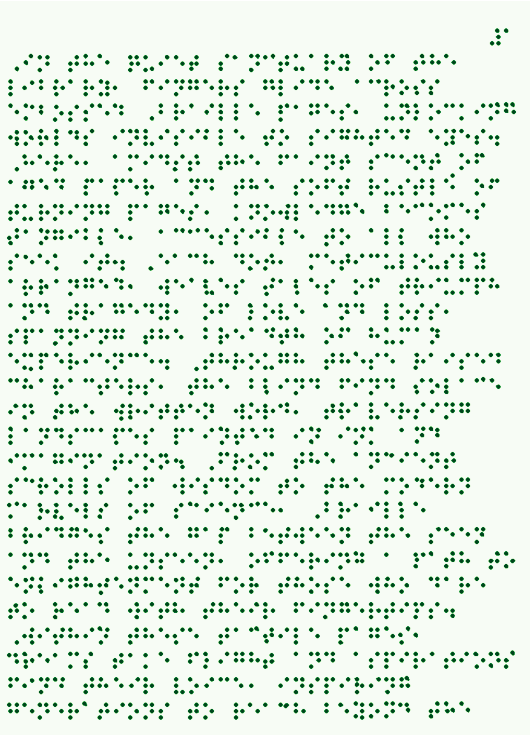
\includegraphics[width=0.55\linewidth]{Hough/Hough.png}}\hfill
    \subfloat[Some of the detected coordinates]{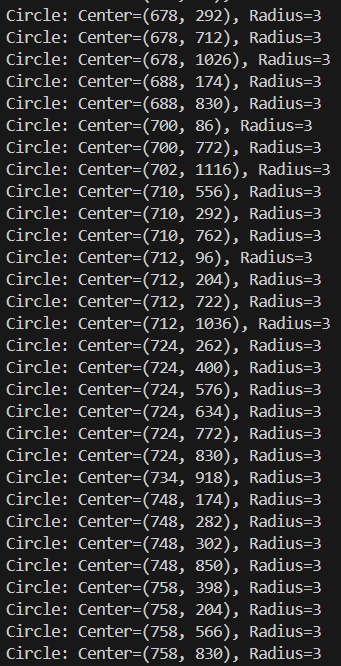
\includegraphics[width=0.39\linewidth]{Hough/snippent.png}}\\
    \caption{Hough Gradient Applied to the edge-detected Braille page}
    \label{fig:num3}
\end{figure}

\subsubsection{Identifying Braille Symbols}
In this section, we will cover the methods used to categorize dot locations stored in the Dots Locations Array. This involves several steps:
1. Sorting the Dots Locations Array: Sorted in ascending order based on X-coordinates.
2. Identifying all unique X-coordinate and Y-coordinate values containing potential dots: To mitigate potential shifts in dot centers, in cases where two unique X-coordinates or Y-coordinates closely align within a specified threshold, the higher X-coordinates or Y-coordinates are excluded, and \textbf{the corresponding dots are aligned with the lower coordinate values}, as shown in figure \ref{fig:num4}. These aligned dots locations are saved in an array that will be mentioned later as \textbf{"Aligned Locations Array"}.

\begin{figure}[H]
    \centering
    \subfloat[Before Alignment]{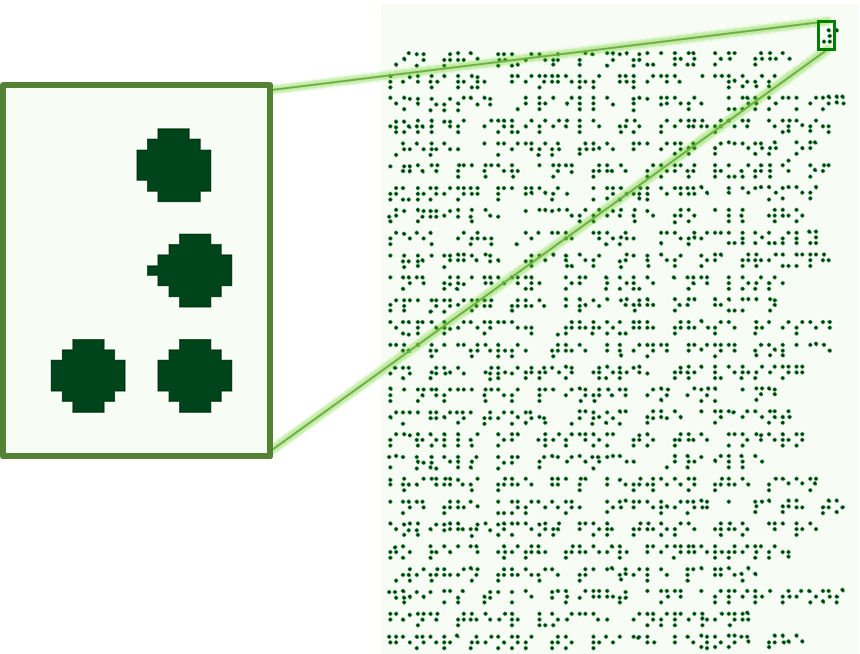
\includegraphics[width=1\linewidth]{Hough/Notalligned.png}}\\
    \subfloat[After Alignment]{\includegraphics[width=1\linewidth]{Hough/Alligned.png}}\\
    \caption{Alignment Applied to the Braille Page.}
    \label{fig:num4}
\end{figure}


\subsubsection{A Challenge: Eliminating Unnecessary Extra Points}

One of the challenges we faced during the process was dealing with Braille Special Characters. These characters are composed of 8 dots instead of 6, and they are not globally used in formal Braille language. However, some of the Braille language users tend to abstract some of their frequently used words, signs, or expressions into one of these 8 dots symbols. Figure \ref{fig:num7} illustrates an example of an 8 dots special Braille symbol.

\begin{figure}[H]
    \centering
    \includegraphics[width=0.25\linewidth]{Hough/8dots.png}
    \caption{8 dots special Braille symbol}
    \label{fig:num7}
\end{figure}

A couple of the sample pages we worked on while building our project had one of these special symbols, as shown in figure 5.6. As these symbols are not globally used and depend on user-based mapping, we decided to ignore the extra dot at any of the very bottom positions and deal with the character as a 6 dots normal symbol. This will definitely result in an incorrect character, but it will be probably corrected in the text correction stage (will be discussed in chapter 7).

\begin{figure}[H]
    \centering
    \includegraphics[width=0.85\linewidth]{Hough/Extra dot.png}
    \caption{8 dots special Braille symbol in on of the sample pages}
    \label{fig:num8}
\end{figure}


\subsection{Recognition}
In this section, we will cover the methods used to convert dot coordinates for each symbol into a binary combination of 6 dots. This process consists of 2 steps: Predicting Potential Dot Locations, and Mapping Braille Symbols into Binary. In the following subsections we will discuss the details of each step.

\subsubsection{Predicting Potential Dot Locations}
In this subsection, we will explain how the potential dot locations were predicted based on the detected dot locations. Following the alignment discussed in section 5.1.3, the program utilizes all unique X-coordinates and Y-coordinates to construct a matrix, where each element represents a potential dot space. The matrix elements are structured such that groups of six elements correspond to individual characters. These predictions are based on the aligned dot coordinates array.

To deliver the idea in a simpler way, assume each dot can be represented with an X-axis and a Y-axis passing through its center. Applying this assumption to all of the dots, \textbf{A virtual grid} is created as illustrated in figure \ref{fig:num5}(a). Red dots represent potential dots locations. \textbf{RED DOTS ARE JUST FOR ILLUSTRATION, THEY ARE NOT A PART OF THE ORIGINAL PAGE.} At each and every intersection, there should be a potential dot location. Based on this concept, a matrix is created, called \textbf{"General Matrix"}, including all of the potential dots locations. This means that the matrix size is MxN where M is the number of symbols rows and N is the number of symbols columns. Each element in the matrix has a size of 1x6, as there are 6 potential dots for each symbol. Figure \ref{fig:num5}(b) represents the potential dots locations in the first row of the page as a sample of the matrix. Figure \ref{fig:num9} illustrates all of the potential dots locations saved in General Matrix.

\begin{figure}[H]
    \begin{adjustwidth}{-2.5cm}{}
        \centering
        \subfloat[Virtual Grid Based on Aligned Dot Coordinates array]{\includegraphics[width=1.1\linewidth]{Hough/Grid.png}}\\
        \subfloat[Potential dots locations in the 1st row in the page]{\includegraphics[width=1.1\linewidth]{Hough/image.png}}\\
    \end{adjustwidth}
    \caption{Potential Dots Prediction}
    \label{fig:num5}
\end{figure}

Currently, it should be clear enough why we assumed that the page should be full of symbols at the very beginning of this chapter. It is because the accuracy of predicting all of the potential dots locations is directly proportional to number of symbols present in a single Braille page. This means, for a page that barely contains symbols, the virtual grid wouldn't fully form. Therefore, the General Matrix wouldn't be fully filled and the recognition process would lack accuracy.
\begin{figure}[H]
    \centering
    \includegraphics[width=0.8\linewidth]{Hough/red.jpg}
    \caption{All of the potential dots locations saved in General Matrix}
    \label{fig:num9}
\end{figure}

\subsubsection{Identifying Braille Symbols and Mapping Braille Symbols into Binary}

The next step is to identify Braille symbols. In order to do this, We're masking the Aligned Locations Array mentioned in section 5.1.3 on the General Matrix mentioned in the previous section. The masking process is illustrated in figure \ref{fig:num8}.  All of the red dots overlapping with green dots represent 1s, while all of the red dots overlapping with empty spaces represent 0s. With the fact that the General Matrix is already symbolized, The Aligned locations array is going to be symbolized and binary mapped after masking into a new array named \textbf{"Updated Symbols"}. Updated symbols array contains multiple rows, where each row contains multiple symbols, where each symbols contains 6 binary values, where ones represent that there is a present dot and zeros represent that there is no dot. Figure \ref{fig:num6} shows the first element of the Updated Symbols array, which represents the first row of the page after being symbolized and mapped to binary.

\begin{figure}[H]
    \begin{adjustwidth}{-1.5cm}{}
      \centering
      \includegraphics[width=1.12\linewidth]{Hough/mask.jpg}
    \end{adjustwidth}
    \caption{Masking Process}
    \label{fig:num8}
\end{figure}

\begin{figure}[H]
    \begin{adjustwidth}{-2.5cm}{}
        \centering
        \includegraphics[width=1.12\linewidth]{Hough/image1.png}
    \end{adjustwidth}
    \caption{1st row of the page after being symbolized and mapped to binary}
    \label{fig:num6}
\end{figure}

The next key step is to simply to translate every symbol into its corresponding alphabetic letter. This step will be discussed in detail later in chapter 7 .


%********************************%
%***********SECTION 6************%
%********************************%
\newpage
\section{Detection Using White Spaces and Recognition Using CNN}

\setcounter{figure}{0}
\renewcommand{\thefigure}{6.\arabic{figure}}

\subsection{Detection}
For the CNN methods the detection process is very important as it provides the CNN model with an image for every character in the page to be translated, this is done by the manipulation of pixels color information providing a reliable dividing process. 
\subsubsection{Turning the image into zeros and ones}
After the preprocessing stage the output page consists of black and white colors only, the value of each pixel is extracted from the page forming a 2D array the same size of the page to be translated, each cell contains either value 1 if the corresponding pixel is black or 0 if the corresponding pixel is white.
\begin{figure}[!ht]
    \centering
    \subfloat[Input demo image]{\includegraphics[width=0.5\linewidth]{6.1.1.png}}\hfill
    \subfloat[2D array of the input image]{\includegraphics[width=1\linewidth]{6.1.13.png}}\\
    \caption{Making a 2D array of zeros and ones from the input image}
    \label{fig:Making a 2D array of zeros and ones from the input image}
\end{figure}

\subsubsection{Determining the existence of black pixels}
The values of cells for each row are summed up and for each column. That gives us the information about which row and which column may have a black pixel.
\subsubsection{Deciding the candidate coordinates}
A suitable constant threshold is selected for the configuration we are working with. The threshold is used for the elimination of rows and columns that contains noise or not enough numbers of black pixels. This gives us the coordinates of the rows and columns which contains a convenient  number of black pixels, and we assign a value for that coordinate.

\clearpage
\begin{figure}[!ht]
\centering
\includegraphics[width=1\linewidth]{6.1.3.png}
\caption{Rows coordinates array after assigning values}
\label{fig:rows coordinates array after assigning values}
\end{figure} 
Using the variance of that value we could determine the coordinate where the whole black dot started and the coordinate where it ended, we utilize these coordinates by taking a step left or right in case of column or a step up and down in case of rows by specific amount determined by the dynamic of coordinates variance to determine every row and column that is a start of a whole braille dot or the end of it.
\begin{figure}[!ht]
\centering
\includegraphics[width=0.7\linewidth]{6.1.4.png}
\caption{Selecting columns and rows coordinate surrounding braille dots}
\label{fig:selecting columns and rows coordinate surrounding braille dots}
\end{figure} 
\begin{figure}[!ht]
    \centering
    \subfloat[selected columns surrounding braille dots (purple is shared coordinate)]{\includegraphics[width=0.4\linewidth]{6.1.5.png}}\hfill
    \subfloat[selected rows surrounding braille dots]{\includegraphics[width=0.4\linewidth]{6.1.6.png}}\\
    \caption{Selected rows and columns surrounding braille dots}
    \label{fig:Selected rows and columns surrounding braille dots}
\end{figure}

\subsubsection{Extracting symbols coordinates}
As each braille symbol contain three rows and two columns, we select the coordinates that contain the whole braille symbol not just a dot by jumping 4 coordinates in case of rows and 2 coordinates in case of columns.
\begin{figure}[!ht]
    \centering
    \subfloat[symbols coordinates array]{\includegraphics[width=0.3\linewidth]{6.1.7.png}}\hfill
    \subfloat[selected coordinates surrounding braille symbols]{\includegraphics[width=0.6\linewidth]{6.1.8.png}}\\
    \caption{Extracting symbols coordinates}
    \label{fig:Extracting symbols coordinates}
\end{figure}

\newpage
\subsubsection{Dividing the page into symbol images}
By iterating the coordinates we extracted from the previous step we iterate each symbol by the four coordinates that holds it, then the images are cropped and passed to the next stage of recognition in order. The dividing was not efficient in case of rotated pages as the process of aligning changed the size of the dots which the threshold is calibrated on, resulting incorrect divisions for some lines, which lead to use of straightened pages only with the CNN approach.

\begin{figure}[!ht]
\centering
\includegraphics[width=1\linewidth]{6.1.9.png}
\caption{samples of divided braille symbols from the first rows of a page}
\label{fig:samples of divided braille symbols from the first rows of a page}
\end{figure} 

\subsubsection{Problems and Challenges }
\paragraph{Eliminating unnecessary Extra points }\par
there are some occasions where the user differentiate from the standard form of the Braille symbol and print the symbol with 4 rows instead of 3, which results in ruining the whole order of the coordinates as we work with only the standard form of 6 Braille dots. This was solved by eliminating the Extra points from the array either by the threshold and considering it as noise or by calculating the distance between it and the previous row, as the first row after three rows should have a bigger distance than the fourth row.
\begin{figure}[!ht]
\centering
\includegraphics[width=0.35\linewidth]{6.1.10.png}
\caption{the variation of vertical distances between fault and normal dots}
\label{fig:the variation of vertical distances between fault and normal dots}
\end{figure} 

\paragraph{Page number fading with threshold}\par
this problem occur as the symbol of the number is always in a whole number of rows alone with no other symbols, so threshold that eliminate noise remove it. To solve this we implemented dynamic threshold, it starts small at the top of the page to pass the number symbol then it returns to the constant threshold which is suitable for the rest of the page.


\begin{figure}[!ht]
\centering
\includegraphics[width=0.8\linewidth]{6.1.11.png}
\caption{the page number symbol in a whole line }
\label{fig:the variation of vertical distances between fault and normal dots}
\end{figure} 








\subsection{Datasets}
In our project, we used two different datasets: one was downloaded from the Kaggle website [15], and the other was created by us. This section will discuss the domains of these datasets.
\subsubsection{Kaggle Dataset}
\begin{enumerate}
    \item \textbf{Description:} 
    This dataset was sourced from the Kaggle website and has been utilized in numerous projects. It comprises images of 26 characters, each represented by 60 images of size 28x28 pixels, with various augmentations (including different shifts, rotations, and brightness values). The labels for the images are the letters from A to Z.
    \item \textbf{Samples:}
    Figures \ref{fig:data1}(a), \ref{fig:data1}(b), \ref{fig:data1}(c), and \ref{fig:data1}(d) show the symbol representing the letter A with different augmentations in this dataset.

\begin{figure}[!ht]
\centering
\subfloat[Brightness changed.]{\includegraphics[width=0.45\linewidth]{brightness.jpg}}\hfill
\subfloat[Shifted.]{\includegraphics[width=0.45\linewidth]{shift.jpg}}\\
\subfloat[Rotated 45 degrees]{\includegraphics[width=0.45\linewidth]{rot1.jpg}}\hfill
\subfloat[Rotated -90 degrees]{\includegraphics[width=0.45\linewidth]{rot2.jpg}}
\caption{Letter A in Braille}
\label{fig:data1}
\end{figure}

    \item \textbf{Problems:}
    \begin{enumerate}
        \item The dataset does not cover all possible combinations of Braille characters.
        \item Some images are rotated at large angles or flipped, causing symbols to resemble others, which decreases the model's accuracy.
        \item The most significant issue is that symbols detected from an entire Braille-written page appear very different from the images in the dataset, preventing the model from recognizing them.
    \end{enumerate}

\end{enumerate}

To overcome these issues, we decided to create our own dataset.

\subsubsection{Custom Dataset}
To obtain a dataset that meets our needs, we created our own dataset using the detection of symbols with white spaces as discussed in the previous section.

\begin{enumerate}
    \item \textbf{Description:} 

    To generate this dataset we used four Braille one-sided pages and we conducted two trials. In the first trial, we used detection in image processing, as discussed in Chapter Five, which produced labeled images for each character. However, we did not use this dataset because the properties of the generated images did not match those of the images that would be used with the model.
    
    In the second trial, we used detection using white spaces, as discussed in the previous section. This method generated unlabeled images, which we then labeled manually. The properties of these images closely matched what we needed. Therefore, the dataset was generated from the second trial.

    
    Initially, the dataset was unbalanced; some symbols had many images while others had only one. To address this imbalance, we applied data augmentation techniques. We augmented the images by shifting, changing brightness, and rotating them at small angles not exceeding 10 degrees to avoid altering the symbol’s shape, among other methods. After augmentation, the dataset comprised 6519 images, with each symbol represented by about 100 images of size 224x224 pixels.The images were labeled as zeros and ones, corresponding to the arrangement of dots as illustrated in the introduction in chapter 1.
        
    \item \textbf{Samples:}
Figures \ref{fig:data}(a), \ref{fig:data}(b), \ref{fig:data}(c), and \ref{fig:data}(d) are samples from our dataset. Figure \ref{fig:data}(a) represents the space, while figures \ref{fig:data}(c) and \ref{fig:data}(d) depict the same symbol; however, noise has been added to the second image.

\begin{figure}[!ht]
\centering
\subfloat['000000']{\includegraphics[width=0.45\linewidth]{2_000000_1.png}}\hfill
\subfloat['010011']{\includegraphics[width=0.45\linewidth]{0_010011_1.png}}\\
\subfloat['001111']{\includegraphics[width=0.45\linewidth]{4_001111.png}}\hfill
\subfloat['001111' with noise]{\includegraphics[width=0.45\linewidth]{4_001111_1.png}}
\caption{Samples from Custom dataset}
\label{fig:data}
\end{figure}
\end{enumerate}

\subsection{Convolutional Neural Network Models}

\begin{figure}
\centering
\includegraphics[width=\linewidth]{cnn.PNG}
\caption{CNN architecture}
\label{fig:cnn}
\end{figure}

A Convolutional Neural Network (CNN or ConvNet) is a class of neural networks that specializes in processing data with a grid-like topology, such as images. A digital image is a binary representation of visual data, consisting of pixels arranged in a grid. Each pixel contains values that indicate its brightness and color. A typical CNN comprises three types of layers: convolutional layers, pooling layers, and fully connected layers as shown in Figure \ref{fig:cnn}

\begin{enumerate}
    \item \textbf{Convolution Layer:} The convolution layer is the core building block of the CNN. It carries the main portion of the network’s computational load.
    \item \textbf{Pooling Layer:} The pooling layer replaces the output of the network at certain locations by deriving a summary statistic of the nearby outputs. This helps in reducing the spatial size of the representation, which decreases the required amount of computation and weights. The pooling operation is processed on every slice of the representation individually.
    \item \textbf{Fully Connected Layer:} Neurons in this layer have full connectivity with all neurons in the preceding and succeeding layers, similar to what is observed in regular Fully Connected Neural Networks (FCNN). Consequently, it can be computed as usual through matrix multiplication followed by the addition of a bias term. The Fully Connected (FC) layer helps map the representation between the input and the output.
    \item \textbf{Non-Linearity Layers:} Since convolution is a linear operation and images are far from linear, non-linearity layers are often placed directly after the convolution layer to introduce non-linearity to the activation map.
\end{enumerate}

This is a brief explanation of Convolutional Neural Networks (CNNs) in general. In the following sections, we will focus on the specific models we used: one model that we built ourselves, and another that utilized a pretrained model called DenseNet201.

\subsubsection{Custom Model}
In this section, we describe the architecture and design of the model built by ourselves. 
\begin{enumerate}
    \item \textbf{Model architecture:} Our model, constructed using the Keras Sequential API, includes the following layers, as illustrated in the block diagram in Figure \ref{fig:custom model}:

\begin{figure}[!ht]
\centering
\subfloat[The complete model]{\includegraphics[width=\linewidth]{model.jpg}}\hfill
\subfloat[First Convolutional Block]{\includegraphics[width=0.45\linewidth]{first block.PNG}}\\
\subfloat[Second,third \& forth Convolutional Blocks]{\includegraphics[width=0.45\linewidth]{second.PNG}}\hfill
\subfloat[Fully Connected Layers]{\includegraphics[width=\linewidth]{fullyconnected.PNG}}
\caption{Custom model block diagram}
\label{fig:custom model}
\end{figure}


    \begin{enumerate}
        \item Input Layer: The input layer is configured to accept grayscale images with a shape of 224x224 pixels and a single color channel.
        
        \item First Convolutional Block:

        \textbf{Conv2D Layer:} 64 filters, 5x5 kernel size, 'same' padding, ReLU activation, and L2 regularization to prevent overfitting.
        
        \textbf{BatchNormalization:} Normalizes the outputs of the convolutional layer to speed up training and improve stability.
        
        \item Second Convolutional Block:

        \textbf{Conv2D Layer:} 64 filters, 3x3 kernel size, 'same' padding, ReLU activation, and L2 regularization.
        
        \textbf{BatchNormalization:} Normalizes the outputs of the convolutional layer.
        
        \textbf{MaxPooling2D:} Reduces the spatial dimensions of the feature maps.
        
        \item Third Convolutional Block:

        \textbf{Conv2D Layer:} 64 filters, 3x3 kernel size, 'same' padding, ReLU activation, and L2 regularization.
        
        \textbf{BatchNormalization:} Normalizes the outputs.
        
        \textbf{MaxPooling2D:} Further reduces the spatial dimensions.
        
        \item Fourth Convolutional Block:

        \textbf{Conv2D Layer:} 64 filters, 3x3 kernel size, 'same' padding, ReLU activation, and L2 regularization.
        
        \textbf{BatchNormalization:} Normalizes the outputs.
        
        \textbf{MaxPooling2D:} Further reduces the spatial dimensions.
        
        \item Flatten Layer:Flattens the output of the convolutional layers into a one-dimensional vector to prepare it for the fully connected layers.
        
        \item Fully Connected Layers:

        \textbf{Dense Layer 1:} 576 neurons with ReLU activation and L2 regularization.
        
        \textbf{BatchNormalization:} Normalizes the outputs.
        
        \textbf{Dropout Layer 1:} 60\% dropout rate to mitigate overfitting.
        
        \textbf{Dense Layer 2:} 288 neurons with ReLU activation and L2 regularization.
        
        \textbf{BatchNormalization:} Normalizes the outputs.
        
        \textbf{Dropout Layer 2:} 40\% dropout rate.
        
        \item Output Layer: The output layer consists of 64 neurons with sigmoid activation, suitable for multi-label classification tasks where each class is independent.
        
    \end{enumerate}

      \item \textbf{Training the model:}
  We trained our model using a custom dataset, carefully dividing the data into 80\% for training and 20\% for testing. The model underwent rigorous training over 1000 epochs, with early stopping implemented to prevent overfitting. This approach ensured that the model was well-tuned and able to generalize effectively, leveraging the comprehensive training data while maintaining robust performance on the testing set.

   \item \textbf{Model Performance:}

   The model scored a test accuracy of 97\% . Figures 6.13 \& 6.14 show the fitting history.
        

\end{enumerate}

   \begin{figure}[H]
        \centering
        \includegraphics[]{cnn_loss_history.png}
        \caption{Model Loss (categorical cross entropy)}
        \end{figure}

    \begin{figure}[H]
        \centering
        \includegraphics[]{cnn_acc_history.png}
        \caption{Model Accuracy}
        \end{figure}
        
\subsubsection{DenseNet201}
In this section, we describe the architecture and design of the neural network model used in our project, which leverages a pretrained DenseNet201 model.
\begin{enumerate}

    \item \textbf{Model architecture:}
    
    \begin{enumerate}
    \item \textbf{Base model (DensNet 201)}
    DenseNet-201 is a convolutional neural network (CNN) architecture that is part of the DenseNet family. The “201” signifies that this particular network has 201 layers.It pretrained on the ImageNet dataset. DenseNet stands for Densely Connected Convolutional Networks, and these networks are known for connecting each layer to every other layer in a feed-forward fashion.
    
    In DenseNet-201, each layer receives additional inputs from all preceding layers and passes on its own feature-maps to all subsequent layers. This creates a highly dense network of connections, with the main benefit being improved flow of information and gradients throughout the network, which makes it efficient in terms of computation and memory usage compared to other deep architectures.
    
    DenseNets are particularly good at solving problems related to image recognition, and they have been shown to achieve excellent performance on benchmark datasets.
    
    The specific steps involved in setting up this base model to use it are as follows:
        \begin{enumerate}
        \item {Loading the DenseNet201 Model:} We loaded the model with specific parameters: weights , input size , include top (Excludes the top classification layer, allowing us to add custom layers for our specific task).

        \item {Freezing Layers:} All layers in the base model are initially frozen, meaning their weights will not be updated during training. This allows us to retain the pretrained feature extraction capabilities.

        \item {Unfreezing the Last 40 Layers:} The last 40 layers of the base model are unfrozen to fine-tune these layers during training. This strikes a balance between leveraging pretrained knowledge and adapting the model to our specific dataset.
        \end{enumerate}

        \item \textbf{Custom Layers:}  After setting up the base model, we add several custom layers to tailor the network for our classification task:

        \begin{enumerate}
            \item Global Average Pooling: This layer reduces the spatial dimensions of the feature maps from the DenseNet201 model, outputting a single 2D vector per feature map.
            \item Fully Connected Layers: 

            \textbf{Dense Layer 1:} 256 neurons with ReLU activation and L2 regularization to prevent overfitting.
            
            \textbf{Dropout Layer 1:} 30\% dropout rate to further mitigate overfitting.
            
            \textbf{Dense Layer 2:} 128 neurons with ReLU activation and L2 regularization.
            
           \textbf{Dropout Layer 2:} 30\% dropout rate.

            \item Output Layer: The output layer consists of 64 neurons with a softmax activation function, suitable for a multi-class classification task with 64 classes.
        \end{enumerate}

        \item \textbf{Model Compilation:} Finally, we compile the model using the Adam optimizer which is known for its efficiency and adaptive learning rate and categorical cross-entropy loss function which is  appropriate for multi-class classification tasks.
        
  \end{enumerate}  
  \item \textbf{Training the model:}
  We trained our model using a custom dataset, carefully dividing the data into 80\% for training and 20\% for testing. The model underwent rigorous training over 1000 epochs, with early stopping implemented to prevent overfitting. This approach ensured that the model was well-tuned and able to generalize effectively, leveraging the comprehensive training data while maintaining robust performance on the testing set.

   \item \textbf{Model Performance:}
   Figure \ref{fig:acc} shows the model's accuracy on the validation and the training set. It's noticeable that the model starts to reach a good performance starting from epoch 60. The training process automatically early-stops at epoch 82 since no further improvement in the model's accuracy occurs.

\begin{figure}
\centering
\includegraphics[]{acc.png}
\caption{Model Accuracy}
\label{fig:acc}
\end{figure}

Figure \ref{fig:loss} shows the model's loss. We have used categorical cross entropy as our loss metric. From figures \ref{fig:acc}  and \ref{fig:loss} we notice no signs of over-fitting, indicating that the model can generalize well on unseen data.

\begin{figure}
\centering
\includegraphics[]{loss.png}
\caption{Model Loss (categorical cross entropy)}
\label{fig:loss}
\end{figure}
For the training data as shown in Table 6.1 , the model achieved an accuracy of 1.00, correctly classifying all 5215 instances in the dataset. The macro average precision, recall, and F1-score are all 1.00, indicating that the model performs exceptionally well across all classes without any bias. Similarly, the weighted average precision, recall, and F1-score are also 1.00, providing a balanced view of the model's performance by considering the number of instances in each class. These perfect scores highlight the model's robustness and reliability in classifying the training data accurately and effectively.

For the testing data as shown in Table 6.2, the model achieved an accuracy of 0.99, correctly classifying 99\% of the 1304 instances in the testing dataset. The macro average precision, recall, and F1-score are all 0.99, demonstrating high accuracy across all classes, similar to the training data performance. The weighted average precision, recall, and F1-score are also 0.99, confirming that the model performs well across all classes when accounting for the number of instances in each class. These near-perfect scores underscore the model's effectiveness and consistency in classification tasks, maintaining high accuracy in both training and testing phases.

\setcounter{table}{0}
\renewcommand{\thetable}{6.\arabic{table}}
\begin{table}
\centering
\begin{tblr}{
}
 & Precision & Recall & F1 score & Support \\
accuracy &           &        &      1    &  5215       \\
 Macro avg &      1     &      1  &    1      &   5215      \\
 Weighted avg &  1         &    1    &   1       &     5215    
\end{tblr} 
\label{tab:table1}
\caption{Model performance on training data}

\end{table}

\begin{table}
\centering
\begin{tblr}{
}
 & Precision & Recall & F1 score & Support \\
accuracy &           &        &      0.99    &  1304       \\
 Macro avg &      0.99     &      0.99  &    0.99      &   1304      \\
 Weighted avg &  0.99         &    0.99    &   0.99       &     1304    
\end{tblr} 
\caption{Model performance on testing data}
\label{tab:table2}
\end{table}


\end{enumerate}





%********************************%
%***********SECTION 7************%
%********************************%
\newpage
\input{Sections/Translation, Correction And Text to Speech}



%********************************%
%***********SECTION 8************%
%********************************%
\newpage

\setcounter{figure}{0}
\renewcommand{\thefigure}{8.\arabic{figure}}
\section{GUI}
 We designed an application that provides a graphical user interface (GUI) designed to facilitate the translation to Braille text from images, with additional features for generating speech output. This document outlines the components and functionality of the GUI, emphasizing its accessibility for visually impaired users. The application is built to run on both Windows 10 and Windows 11. However, it can be adjusted to be built on Linux as well.

\subsection{Design Features}


\begin{itemize}
    \item \textbf{Central Widget}: This widget serves as the main container for the GUI elements.
    
    \item \textbf{Stacked Widget}: Used to manage different pages within the GUI.
    
    \begin{itemize}
        \item \textbf{Page 1 - Initial Translation Options:}: The initial screen allows users to select their translation options, such as translating multiple images, a single image, or enabling speech generation.

        \begin{figure}[h!]
            \centering
            \includegraphics[width=0.6\textwidth]{main_page.png}
            \caption{Design layout of Page 1 - Initial Translation Options}
        \end{figure}
        
        \begin{itemize}
            \item \textbf{Translate Multiple Pages}: Button to initiate translation of multiple images.
            \item \textbf{Translate One Page}: Button to translate a single image.
            \item \textbf{Voice Generation}: Checkbox for enabling Speech generation.
            \item \textbf{Generate Voice From Text}: Button to generate Speech from translated text.
        \end{itemize}
        
        \item \textbf{Page 2 - Configuration Settings:}: This screen is used for configuring the translation settings, including selecting the type of translation, enabling image processing, choosing AI-based translation, and browsing input files or folders.

        \begin{figure}[h!]
            \centering
            \includegraphics[width=0.6\textwidth]{options_page.png}
            \caption{Design layout of Page 2 - Configuration Settings}
        \end{figure}
        
        \begin{itemize}
            \item \textbf{Direct Translation}: Checkbox for selecting image processing mode.
            \item \textbf{AI Translation}: Checkbox for selecting AI-based translation.
            \item \textbf{Browse}: Button to browse and select input files or folders.
            \item \textbf{Path Label}: Label displaying the selected file or folder path.
            \item \textbf{Return Button}: Button to return to the home screen.
            \item \textbf{Start Button}: Button to start the translation process.
        \end{itemize}
        
        \item \textbf{Page 3 - Audio Playback and Text Display:}: This screen is designed for text display, allowing users to pen generated text and audio files, and view the translated text.

        \begin{figure}[h!]
            \centering
            \includegraphics[width=0.6\textwidth]{result_page.png}
            \caption{Design layout of Page 3 - Text Display}
        \end{figure}
        
        \begin{itemize}
            \item \textbf{Open Translation Results Folder Button}: Button to open the folder containing generated text files and speech audio.
            \item \textbf{Text Display}: Text browser widget to display translated and corrected text.
            \item \textbf{Translate Another}: To translate a new file. This button returns the user back to the main page.
        \end{itemize}
    \end{itemize}
\end{itemize}

\subsection{Tools and Frameworks}
The development of the Optical Braille Translator application GUI leverages various tools and frameworks to ensure efficiency and reliability. Key tools and frameworks include:

\begin{itemize}
    \item \textbf{Qt Designer}: Utilized for creating the graphical user interface with a focus on cross-platform compatibility.
    \item \textbf{OpenCV}: Employed for image processing tasks to detect and translate Braille text from images.
    \item \textbf{TensorFlow}: Used for AI-based translation capabilities, enhancing the accuracy of Braille text recognition.
    \item \textbf{PyQt}: Provides the integration of Python with Qt, facilitating the development of the application in Python. The version used is PyQt5.
\end{itemize}


\subsection{Accessibility Features}

The GUI of the Optical Braille Translator application is designed to be accessible for visually impaired users, adhering to accessibility standards and providing the following features:

\begin{itemize}
    \item \textbf{High Contrast and Custom Styling}: Utilizes high contrast colors and custom styling for improved readability and navigation.
    
    \item \textbf{Text-to-Speech (TTS) Integration}: Enables speech generation from translated text, supporting users who rely on auditory feedback.
    
    \item \textbf{Keyboard Navigation and Screen Reader Compatibility}: Supports keyboard navigation and is compatible with screen readers to assist users with visual impairments in navigating and interacting with the GUI.
\end{itemize}

\newpage
\setcounter{figure}{0}
\renewcommand{\thefigure}{9.\arabic{figure}}
\section{Testing and Results}

This section demonstrates the results obtained from testing the Optical Braille Translator application on multiple Braille pages that fit the specified standards and constraints.

\subsection{Image Processing Detection Results}
The image processing step involves detecting and dividing Braille characters from the input images. The accuracy of this step was evaluated on a set of standardized Braille pages. The results showed a high detection rate for individual Braille dots of 99.8\% in which a total of 10,212 dots were detected out of 10,231 dots. These 19 errors were  found by testing 4 rotated  images and 3 non-rotated. 

The page with the least accuracy, shown in the following figure, has 9 undetected dots  out of 2087 dots. It is important to consider that this image had a rotation angle of  -1.4 degrees while scanning.

\begin{figure}[H]
    \centering  
    \subfloat[rotated scanned image as the input of the system]{\includegraphics[width=0.5\linewidth]{Image (43).jpg}}
    \subfloat[the undetected dots in the page]{\includegraphics[width=0.5\linewidth]{ex22.PNG}}\hfill
  
    \caption{example of the Hough circle transformation used for dot detection }
    \label{fig:num2}
\end{figure}


\subsection{Image Processing Translation Results}
Although we use an AI model for character classification. Our Image Processing algorithm is capable of classifying characters after identifying them as mentioned, leading to a translation accuracy of 97.98\%.  (20 mistakes out of 989 words including punctuation) .This approach can be time efficient as AI classification can be difficult and resource-consuming for some machines.

        \begin{figure}[h!]
            \centering
            \includegraphics[width=0.6\textwidth]{ip.png}
            
            \caption{Image Processing Algorithm Translation: 2 Dashing Mistakes}
        \end{figure}

\subsection{AI Translation Results}
The AI-based translation step classifies the detected Braille characters into the corresponding text. This was tested using a pre-trained model on a diverse set of Braille samples. The AI model demonstrated a high classification accuracy on the test set of 99\%, correctly identifying the majority of the Braille characters.
When tested on 5 images the system gave 94.45\% accuracy. This was achieved by translating 5 wrong words out of 3.



\subsection{Text Correction Results}
Following the AI translation, the text correction step was applied to improve the accuracy of the translated text. This step is crucial as it involves correcting any misclassifications and ensuring that the corrected text adheres to grammatical and syntactical standards while maintaining the context of the translated passage. For this task, we employed the AI Forever T5 spell checker, a model renowned for its robust performance in text correction tasks.

The AI Forever T5 spell checker, which is based on the T5 (Text-To-Text Transfer Transformer) architecture, has shown exceptional capabilities in handling text correction due to its extensive pre-training on a diverse corpus and its sophisticated sequence-to-sequence learning mechanism. This model outperforms previous generation models like GPT-3.5 in several benchmarks, particularly in tasks requiring precise grammatical corrections and context preservation. Further details about the AI Forever T5 model can be found in Chapter 7, Section 2.

In our application, the text correction process achieved an impressive accuracy of 100\%, largely due to the high accuracy of the initial translation step, which minimized the number of errors needing correction. While the AI Forever T5 model has a reported overall accuracy of 83\% in general text correction tasks, our specific use case involved small paragraphs with a limited number of misspelled words. This controlled scenario allowed the model to perform with significantly higher accuracy. The effectiveness of the AI Forever T5 spell checker in our context underscores its capability to handle nuanced and context-sensitive text correction tasks with high precision, making it a valuable tool in our translation and text correction pipeline. The following are some additional example outputs.



\subsubsection*{Example 1}
\begin{itemize}
    \item \textbf{Original Passage}: \textcolor{red}{Th} \textcolor{red}{quikc} \textcolor{red}{borwn} fox \textcolor{red}{jmups} \textcolor{red}{ovre} the \textcolor{red}{lazi} dog.
    \item \textbf{Corrected Passage}: \uline{\textcolor{green}{The}} \uline{\textcolor{green}{quick}} \uline{\textcolor{green}{brown}} fox \uline{\textcolor{green}{jumps}} \uline{\textcolor{green}{over}} the \textcolor{green}{lazy} dog.
    \item \textbf{Misspelled Words}: 6
    \item \textbf{Corrected Words}: 6
    \item \textbf{Accuracy}: 100\%
\end{itemize}

\subsubsection*{Example 2}
\begin{itemize}
    \item \textbf{Original Passage}: I \textcolor{red}{cnnot} \textcolor{red}{beleive} how \textcolor{red}{beautifull} the \textcolor{red}{scenry}is at the \textcolor{red}{moountain.}
    \item \textbf{Corrected Passage}: I \uline{\textcolor{green}{cannot}} \uline{\textcolor{green}{believe}} how \uline{\textcolor{green}{beautiful}} the \uline{\textcolor{green}{scenery}} is at the \uline{\textcolor{green}{mountain.}}
    \item \textbf{Misspelled Words}: 5
    \item \textbf{Corrected Words}: 5
    \item \textbf{Accuracy}: 100\%
\end{itemize}

\subsubsection*{Example 3}
\begin{itemize}
    \item \textbf{Original Passage}: \textcolor{red}{Plase} \textcolor{red}{remmber} to bring \textcolor{red}{yoor} \textcolor{red}{umberela} \textcolor{red}{tomorow} \textcolor{red}{becase} it will rain.
    \item \textbf{Corrected Passage}: \uline{\textcolor{green}{Please}} \uline{\textcolor{green}{remember}} to bring \uline{\textcolor{green}{your}} \uline{\textcolor{green}{umbrella}} \uline{\textcolor{green}{tomorrow}} \uline{\textcolor{green}{because}} it will rain.
    \item \textbf{Misspelled Words}: 6
    \item \textbf{Corrected Words}: 6
    \item \textbf{Accuracy}: 100\%
\end{itemize}




\subsection{Overall Accuracy}
The overall accuracy of the Optical Braille Translator application was evaluated by combining the results of image processing, AI translation, and text correction. The performance metrics for each step and the cumulative accuracy are presented in the table below.

\begin{table}[h!]
    \centering
    \begin{tabular}{|l|c|}
        \hline
        \textbf{Process} & \textbf{Accuracy (\%)} \\
        \hline
        Detecting dots by image processing & 99.8\% \\
        \hline
        Classification of characters using AI model & 99\% \\
         \hline
        Word translation accuracy (Image Processing Algorithm) & 97.98\% \\
        \hline
        Word translation accuracy (AI Model) & 94.45\%\\
       
        \hline
        Correction accuracy & 100\% \\
        \hline
       
    \end{tabular}
    \caption{Accuracy results for different steps of the Optical Braille Translator application}
\end {table}

\subsection{Translation Speed}
The benefit of using image processing is most obvious when observing the speed of the different processes.  the system can finish all the image processing steps in under 1 second.  This includes filters, dot detection, grid formation, or white spaces detection  technique.  for example, one full page as an input scanned image to an output of non-corrected text takes 0.7 seconds to be processed.
On the other hand, AI models are not as fat because, as previously mentioned, they are resource-consuming and their performance varies from one machine to another.

\begin{table}[h!]
    \centering 
    \begin{tabular}{|l|p{3cm}|p{3cm}|p{3cm}|}
        \hline
        \textbf{User} & \textbf{Text Generation (seconds)} & \textbf{Text Correction (seconds)} & \textbf{Total Time (seconds)} \\
        \hline
        HP ProBook & 180 & 150 & 330 \\
        \hline
        Google Colab & 153 & 49 & 202 \\
        \hline
        Kaggle & 130 & 38 & 168 \\
        \hline
        ASUS TUF Gaming F17 & 91 & 30 & 121 \\
        \hline
    \end{tabular}
    \caption{Translation time for multiple users for one braille page}
    \label{tab:translation-times}
\end{table}


%********************************%
%***********SECTION 9************%
%********************************%
\newpage
\section{Conclusion and Future Work}
\subsection{Conclusion}
The "Braille Translator" project addresses a significant gap in accessibility for visually impaired individuals by providing a system that translates Braille into English text and converts it into audible speech. This innovation enhances access to Braille content and supports literacy and independence for those with visual impairments.

Braille literacy is a fundamental skill that empowers individuals with visual impairments to read and write independently. However, the traditional processes of converting printed text into Braille and vice versa are labor-intensive and inaccessible to those who are not proficient in Braille. This project aims to mitigate these challenges by developing a system that leverages image processing and deep learning techniques to translate scanned Braille images into English text, further converting this text into speech to make Braille content accessible to everyone.

The project's primary objectives were to accurately detect and recognize Braille characters from scanned images and to convert the recognized text into audible speech. Through a multi-step approach, including image preprocessing with an accuracy of 97.98\%, character detection and recognition using convolutional neural networks (CNNs) with an accuracy of 94.45\%, text correction with an accuracy of 100\%, and text-to-speech conversion, achieves these goals. The development of a user-friendly graphical user interface (GUI) ensures ease of use, and extensive testing confirms the system's performance and accuracy.

By translating grade 1, front-only, scanned Braille images into coherent English text and providing auditory output, the "Braille Translator" system significantly enhances accessibility for visually impaired individuals. This project not only supports Braille literacy but also bridges the gap for those without Braille skills, enabling them to access and interact with Braille content effortlessly.

In conclusion, the "Braille Translator" project demonstrates the potential of technology to improve the lives of visually impaired individuals. By combining image processing, deep learning, and text-to-speech technologies, the system provides an innovative solution to the challenges of Braille accessibility. This project is a testament to the power of interdisciplinary approaches in creating inclusive technologies that promote literacy, independence, and equality for all.




\newpage

\subsection{Future Work}
\quad Since image processing and AI are continuously evolving, it is crucial to enhance our tools and programs accordingly. We have outlined a plan to improve our project in the following ways:
\begin{enumerate}
    \item \textbf{Enhancing AI Recognition Accuracy and Add Symbol Detection using AI models}:
    \begin{itemize}
        \item Improve the accuracy of the AI model to ensure better Braille translation results.
        \item Incorporate AI-based symbol detection to enhance the recognition of various Braille symbols and special characters.
    \end{itemize}
    
    \item \textbf{Generalization of Image Processing}:
    \begin{itemize}
        \item Develop and implement more robust image processing algorithms capable of handling a wider range of orientations and increased levels of noise.
        \item Ensure the system can effectively process images regardless of the angle or condition in which they are scanned or photographed.
    \end{itemize}
    
    \item \textbf{Optimizing Preprocessing Time}:
    \begin{itemize}
        \item Focus on reducing the preprocessing time required for each image while maintaining or improving the functionality and accuracy of the preprocessing steps.
    \end{itemize}
    
    \item \textbf{Handling Double-Sided Pages}:
    \begin{itemize}
        \item Generalize the program to efficiently process and translate double-sided Braille pages, addressing any challenges related to overlapping or mirrored dots.
    \end{itemize}
    
    \item \textbf{Translating Grade-2 Braille}:
    \begin{itemize}
        \item Add a feature to support the translation of Grade 2 Braille, which includes contractions and abbreviations, providing a more comprehensive translation tool for advanced Braille users.
    \end{itemize}
    
    \item \textbf{Multi-Language Translation}:
    \begin{itemize}
        \item Expand the program's capabilities to support translation in multiple languages, making it a versatile tool for users around the world who rely on Braille in different languages.
    \end{itemize}
    
\end{enumerate}









%********************************%
%***********SECTION 10************%
%********************************%
%-------References-------%
\newpage
% Hide this section from the TOC
\addtocontents{toc}{\protect\setcounter{tocdepth}{-1}}

\patchcmd{\thebibliography}{\section*}{\section}{}{}

% Suppress the section number for the References section
\renewcommand\thesection{} 

% Now we need a bibliography:
\begin{thebibliography}{99}

\bibitem{falcon2005}
Falcón, N., Travieso, C., Alonso, J., \& Ferrer, M. (2005). 
 Image Processing Techniques for Braille Writing Recognition. 
 In \textit{Proceedings of the International Conference on Image Analysis and Recognition} (pp. 379-385). Springer. \url{https://doi.org/10.1007/11556985_49}

    \bibitem{antonacopoulos2004}
    Antonacopoulos, A., \& Bridson, D. (2004). 
    A Robust Braille Recognition System. 
    In \textit{Document Analysis Systems VI} (pp. 533–545). Springer.

    \bibitem{al-salman2007}
    Al-Salman, A., AlOhali, Y., AlKanhal, M., \& AlRajih, A. (2007). 
    An Arabic Optical Braille Recognition System. 
    In \textit{Proceedings of the International Conference on Document Analysis and Recognition}.

    \bibitem{isayed2015}
    Isayed, S., \& Tahboub, R. (2015). 
    A Review of Optical Braille Recognition. 
    In \textit{Proceedings of the International Workshop on Systems, Signal Processing and their Applications} (pp. 1-5). IEEE. \url{https://doi.org/10.1109/WSWAN.2015.7210343}

    \bibitem{chamalee2016}
    Chamalee, W., Srilal, N., Athapaththu, H., \& Ranathunga, L. (2016). 
    Novel Segmentation Method for Optical Braille Character Identification. 
    In \textit{Proceedings of the International Conference on Advances in ICT for Emerging Regions}.

    \bibitem{ovodov2020}
    Ovodov, I. (2020). 
    Optical Braille Recognition Using Object Detection CNN. 
    In \textit{Proceedings of the International Conference on Pattern Recognition and Image Analysis}.

    \bibitem{kausar2021}
    Kausar, T., Sajjad, M., Kausar, A., Lu, Y., Muhammad, W., \& Ashraf, M. (2021). 
    Deep Learning Strategy for Braille Character Recognition. 
    \textit{IEEE Access}, \textit{PP}, 1-1. \url{https://doi.org/10.1109/ACCESS.2021.3138240}

    \bibitem{shokat2022}
    Shokat, S., Riaz, R., Rizvi, S., Khan, I., \& Paul, A. (2022). 
    Characterization of English Braille Patterns Using Automated Tools and RICA Based Feature Extraction Methods. 
    \textit{Sensors}, \textit{22}(5), 1836. \url{https://doi.org/10.3390/s22051836}

    \bibitem{elmi2002}
    Elmi, M., \& Evens, M. (2002). 
    Spelling Correction Using Context. 
    In \textit{Proceedings of the Conference on Computational Linguistics} (pp. 1-6). \url{https://doi.org/10.3115/980451.980906}

    \bibitem{arik2017}
    Arik, S., Chrzanowski, M., Coates, A., Diamos, G., Gibiansky, A., Kang, Y., Li, X., Miller, J., Raiman, J., Sengupta, S., \& Shoeybi, M. (2017). 
    Deep Voice: Real-time Neural Text-to-Speech. 
    In \textit{Proceedings of the International Conference on Machine Learning}.

    \bibitem{wang2017}
    Wang, Y., Skerry-Ryan, R.J., Stanton, D., Weiss, R., Jaitly, N., Yang, Z., Xiao, Y., Chen, Z., Bengio, S., Le, Q., Agiomyrgiannakis, Y., Clark, R., \& Saurous, R. (2017).     Tacotron: Towards End-to-End Speech Synthesis.      In \textit{Proceedings of the Annual Conference of the International Speech Communication Association} (pp. 4006-4010). \url{https://doi.org/10.21437/Inters    peech.2017-1452}

    \bibitem{ritchings}
    Ritchings, R., \& Antonacopoulos, A., \& Drakopoulos, D. 
    Analysis of Scanned Braille Documents. 
    In \textit{Proceedings of the International Conference on Document Analysis and Recognition}.

    \bibitem{afb}
    American Foundation for the Blind. 
    \textit{What is Braille?}. Retrieved from \url{https://afb.org/blindness-and-low-vision/braille/what-braille}

    \bibitem{canny}
    Canny Algorithm. 
    Retrieved from \url{https://www.educative.io/answers/what-is-canny-edge-detection}
    
    \bibitem{kaggle}
    Kaggle dataset. 
    Retrieved from \url{https://www.kaggle.com/datasets/shanks0465/braille-character-dataset}

    \bibitem{cnn}
    Convolutional Neural Network. 
    Retrieved from \url{https://towardsdatascience.com/convolutional-neural-networks-explained-9cc5188c4939}

    \bibitem{contextualSpellCheck}
    Python’s ‘contextualSpellCheck’ Package. 
    Retrieved from \url{https://spacy.io/universe/project/contextualSpellCheck}

    \bibitem{t5}
    Pre-trained ‘T5-large-spell’ Model. 
    Retrieved from \url{https://huggingface.co/ai-forever/T5-large-spell}

    \bibitem{opencv}
    Open source computer vision. 
    Retrieved from \url{https://docs.opencv.org/4.x/}
    
\end{thebibliography}

\noindent

\addtocontents{toc}{\protect\setcounter{tocdepth}{1}}






\end{document}